\documentclass[a4paper,12pt,twoside]{report}
\usepackage[english]{babel} 
\usepackage[T1]{fontenc}
\usepackage[utf8]{inputenc}
\usepackage[a4paper, hmarginratio=3:2]{geometry}

\usepackage{amsmath} % balíček pro pokročilou matem. sazbu
\usepackage{amsthm}
\usepackage{amsfonts}
\usepackage{fixltx2e}
\usepackage{rotating}
\usepackage{url}
\usepackage{epstopdf}
\usepackage{lscape}
\usepackage[round]{natbib}
\usepackage{booktabs}
\usepackage{graphicx}
\usepackage{placeins}

\topmargin=-15mm      % horní okraj trochu menší
\textwidth=150mm      % šířka textu na stránce
\textheight=240mm     % "výška" textu na stránce

\pagenumbering{arabic} % číslování stránek arabskými číslicemi
\pagestyle{plain}      % stránky číslované dole uprostřed

\parindent=0pt % odsazení 1. řádku odstavce
\parskip=7pt   % mezera mezi odstavci
\frenchspacing % aktivuje použití některých českých typografických pravidel

\newcommand{\ti}{\textit} %zkrácený příkaz pro kurzívu
\newcommand{\tb}{\textbf} %zkrácený příkaz pro tučné

\newtheorem{nullhypo}{Null Hypothesis}
\newtheorem{alterhypo}{Alternative Hypothesis}
\newtheorem{hypo}{Hypothesis}

%%%%%%%%%%%%%%%%%%%%%% zde jsou zavedeny některé "konstanty" - můžete, resp. musíte je ZMĚNIT %%%%%%%%%%%%%%%%%%%%%%
\newcommand{\cvut}{Czech Technical University}
\newcommand{\fjfi}{Faculty of Nuclear Sciences and Physical Engineering}
\newcommand{\kse}{Department of Software Engineering}
\newcommand{\obor}{Engineering Informatics}
\newcommand{\zamereni}{Applied Software Engineering}

\newcommand{\nazevcz}{Navigování ve virtuálním světě}        % zde VYPLŇTE český název práce (přesně podle zadání!)
\newcommand{\nazeven}{Navigation in virtual environment}     % zde VYPLŇTE anglický název práce (přesně podle zadání!)
\newcommand{\autor}{Bc. Václav Honzík}           % zde VYPLŇTE své jméno a příjmení
\newcommand{\rok}{2014}                % zde VYPLŇTE rok odevzdání, např. 2006
\newcommand{\vedouci}{Doc. Ing. Zdeněk Žabokrtský, Ph.D.}         % zde VYPLŇTE jméno a příjmení vedoucího práce, včetně titulů
                                                               % např. Doc. Ing. Ivo Malý, Ph.D.
\newcommand{\pracovisteVed}{Institute of Formal and Applied Linguistic, Faculty of
Mathematics and Physics, Charles University in Prague} % zde VYPLŇTE pracoviště vedoucího práce, je-li jiné než KSE FJFI ČVUT

\newcommand{\konzultant}{Prof. Kristina Striegnitz, Ph.D.} % POKUD MÁTE určeného konzultanta, NAPIŠTE jeho jméno a příjmení
\newcommand{\pracovisteKonz}{Union College, Schenectady, NY USA} % POKUD MÁTE konzultanta, NAPIŠTE jeho pracoviště


\newcommand{\klicova}{navigace, odkazující výrazy, jazyková realizace}   % zde NAPIŠTE česky max. 5 klíčových slov
\newcommand{\keyword}{navigation, referring expressions, language realization}       % zde NAPIŠTE anglicky max. 5 klíčových slov (přeložte z češtiny)
\newcommand{\abstrCZ}{Tato práce se zabývá generováním přirozeného jazyka pro navigovaní ve virtuálním světě. Předmětem zájmu jsou zajímavé strategie odkazování, které byly objeveny v dostupných datech v nichž jedna osoba navigovala druhou. Tyto strategie se vymikají běžným metodám v disciplíně generování odkazujících výrazů a tak je tato práce analyzuje a pokouší se je modelovat technikami strojového učení. V rámcí této práce je také proveden experiment studujicí vliv používání těchto strategií na efektivnost navigování. Výsledky naznačují, že tyto strategie jsou přílíš komplexní na to aby mohly být uspěšně modelovány prostorovými informacemi ze scény a musí k tomu být využity i lidské faktory. Experiment ukázal, že strategie DOLPNIT vliv na efektivnost navigování. } % zde NAPIŠTE abstrakt v češtině
\newcommand{\abstrEN}{This thesis discusses a natural language generation in a virtual environment navigational task. It focuses on interesting referencing strategies which was discovered in available dataset of human to human interaction. Because these strategies does not follow common methodology of referring expression generation field, this paper analyses them and attempts to model them using machine learning techniques. It also presents an experiment assessing their effect on the task proficiency. The results suggest that such strategies are too complex to model using spatial information from the scene and human factors must be taken into account. The experiment concludes that they FILL RESULTS effect on the task proficiency.   }                  % zde NAPIŠTE abstrakt v angličtině

\begin{document}


%%%%%%%%%%%%%%%%%%%%%% 1. strana -- na následujících 30 řádků NESAHEJTE!!!  Generuje se AUTOMATICKY %%%%%%%%%%%%%%%%%%%%%%
\thispagestyle{empty}

\begin{center}
    {\Large \textsc{\cvut}\\[1.5ex] \textsc{\fjfi}}\\
    \vspace{10mm}
    
    \begin{tabular}{c}
	    {\bf \kse}\\   
      {\bf Field: \obor}\\
    \end{tabular}


   % logo CVUT -- pokud jej nechcete použít, zakomentujte následující řádek a odkomentujte řádek pod ním:
   %\vspace{10mm} \epsfysize=25mm \epsffile{cvut-logo-bw} \vspace{15mm}
   \vspace{10mm} 
\includegraphics[height=25mm]{cvut-logo-bw} \vspace{15mm}
 
   %\vspace{50mm}

   {\huge \bf \nazeven}\\
   \vspace{5mm}   
   {\huge \bf \nazevcz}
   %{\Huge \bf \nazeven\par}

   \vspace{15mm}
   {\Large MASTER THESIS}

   \vfill
   {\large
    \begin{tabular}{rl}
    Author: & \autor\\
    Supervisor: & \vedouci\\
    Year: & \rok
    \end{tabular}
   }
\end{center}

%%%%%%%%%%%%%%%%%%%%%% 2. strana: zadání práce  %%%%%%%%%%%%%%%%%%%%%%
%%%%%%%%%%%%%%%%%%%%%%            Před svázáním namísto této strany VLOŽÍTE zadání podepsané děkanem!
\newpage  % SEM NESAHEJTE!
\thispagestyle{empty} Insert assignment instead of this page before handing in the thesis!!!!

%%%%%%%%%%%%%%%%%%%%%% 3. strana: prohlášení -- ŽENY UPRAVÍ minulý čas sloves %%%%%%%%%%%%%%%%%%%%%%
\newpage % SEM NESAHEJTE!
\thispagestyle{empty}  % SEM NESAHEJTE!

~ % SEM NESAHEJTE!
\vfill % prázdné místo. SEM NESAHEJTE!

{\bf Declaration} % SEM NESAHEJTE!

\vspace{0.5cm} % vertikální mezera. SEM NESAHEJTE!
I declare, that I have developed my master thesis independently and used only the materials (literature, projects, SW etc.) listed in attached list.

\vspace{5mm}In Prague on ..................\hfill  % SEM NESAHEJTE!
    \begin{tabular}{c}                               % SEM NESAHEJTE!
    ........................................\\       % SEM NESAHEJTE!
    \autor                                           % SEM NESAHEJTE!
    \end{tabular}                                    % SEM NESAHEJTE!



%%%%%%%%%%%%%%%%%%%%%% 4. strana: poděkování -- UPRAVTE JMÉNO, resp. tuto stránku celou VYMAŽTE %%%%%%%%%%%%%%%%%%%%%%
%%%%%%%%%%%%%%%%%%%%%%                           (poděkování nemusí být uvedeno vůbec)
\newpage
\thispagestyle{empty}

~
\vfill % prázdné místo

{\bf Acknowledgment}

\vspace{5mm} % vertikální mezera
I would like to thank \vedouci{} for supervising and shaping my master thesis. I would like to also thank \konzultant{} for giving me the opportunity and helping me with my master thesis.

\begin{flushright}
\autor
\end{flushright}  % <------- tady končí stránka s poděkováním

%%%%%%%%%%%%%%%%%%%%% 5.strana: abstrakt %%%%%%%%%%%%%%%%%%%%%
\newpage   % SEM NESAHEJTE!
\thispagestyle{empty}   % SEM NESAHEJTE!

% příprava:    (na následujících 8 řádků NESAHEJTE!)
\newbox\odstavecbox
\newlength\vyskaodstavce
\newcommand\odstavec[2]{%
    \setbox\odstavecbox=\hbox{%
         \parbox[t]{#1}{#2\vrule width 0pt depth 4pt}}%
    \global\vyskaodstavce=\dp\odstavecbox
    \box\odstavecbox}
\newcommand{\delka}{120mm} % šířka textů ve 2. sloupci tabulky

% použití přípravy:    % dovnitř "tabular" vůbec NESAHEJTE!
\begin{tabular}{ll}
  {\em Title:} & ~ \\
  \multicolumn{2}{l}{\odstavec{\textwidth}{\bf \nazeven}} \\[5mm]
  {\em Author:} & \autor \\[5mm]
  {\em Field:} & \obor \\
  {\em Type of thesis:} & Master thesis \\[5mm]
  {\em Supervisor:} & \odstavec{\delka}{\vedouci \\ \pracovisteVed} \\[5mm]
  {\em Advisor:} & \odstavec{\delka}{\konzultant \\ \pracovisteKonz} \\[5mm]
  \multicolumn{2}{l}{\odstavec{\textwidth}{{\em Abstract:} ~ \abstrEN \\ }} \\[5mm]
  {\em Key words:} & \odstavec{\delka}{\keyword} \\[20mm]

  {\em Název práce:} & ~\\
  \multicolumn{2}{l}{\odstavec{\textwidth}{\bf \nazevcz}}\\[5mm]
  {\em Autor:} & \autor \\[5mm]
%  {\em Obor:} & Inženýrská Informatika \\
%  {\em Typ práce:} & Diplomová práce \\[5mm]
%  {\em Vedoucí:} & \odstavec{\delka}{\vedouci \\ \pracovisteVed} \\[5mm]
%  {\em Konzultant:} & \odstavec{\delka}{\konzultant \\ \pracovisteKonz} \\[5mm]
  \multicolumn{2}{l}{\odstavec{\textwidth}{{\em Abstrakt:} ~ \abstrCZ \\ }} \\[5mm]
  {\em Klíčová slova:} & \odstavec{\delka}{\klicova}
\end{tabular}


%%%%%%%%%%%%%%%%%%%%%% 6. strana: obsah práce ... je generován AUTOMATICKY %%%%%%%%%%%%%%%%%%%%%%
\newpage  % SEM NESAHEJTE!
\tableofcontents % SEM NESAHEJTE!


%%%%%%%%%%%%%%%%%%%%%%  7.strana: zde začíná SAMOTNÁ PRÁCE  %%%%%%%%%%%%%%%%%%%%%%%%%%%%%%%%%%%%%%%%%%%%
%                                 - text se vkládá Z EXTERNÍCH SOUBORŮ
%                                   (můžete ho také napsat přímo sem => smažte každé \input{...})
\newpage % SEM NESAHEJTE!

\chapter*{Introduction} \addcontentsline{toc}{chapter}{Introduction} % SEM NESAHEJTE!
This thesis deals with language generation for navigating in a virtual environment. A dataset of spoken interactions from a shared navigation task is used to model the language generation. The thesis explores a particular strategy of referring, which differs from the traditional methodology used in the relevant research. 

It consists of five chapters.

The first chapter describes the background of the navigation and especially of the language generation in navigation. It introduces the domain of Referring Expression Generation and a related research.

In the second chapter the GIVE framework is introduced. The whole thesis is built upon this framework and it is therefore vital for the following chapters. 

The third chapter introduces the spoken interaction of the S-GIVE dataset. The S-GIVE dataset was created in the GIVE framework and this thesis is one of the first papers to analyse it.

With the fourth chapter starts my contribution. The chapter analyses the S-GIVE dataset and attempts to create models of Natural Language Generation using machine learning techniques. Using the data from the S-GIVE dataset, it explores various sub-problems of language generation.

In the fifth chapter, an experiment to evaluate the mentioned referring strategy is described. Once again built upon the GIVE framework, it compares the newly discovered strategy with more traditional approaches.   

The goals of this thesis are as follows. Analyse the S-GIVE dataset. General statistics, referring expressions and the new referring strategy are the focus of the analysis. Use machine learning techniques to model the referring expression generation in the GIVE scenario. Spatial features are of a particular interest of this thesis. Compare the task efficiency of the new referring strategy with strategy inspired by current research in referring expression generation. The comparison is done through an experiment with human subjects.   % text úvodu (bez nadpisu) je vkládán z jiného souboru; lze upravit jméno souboru, resp. smazat tento řádek a text úvodu napsat přímo sem (ale znepřehlední se to)

% Následují texty kapitol. Smažete-li následující řádky (text chcete psát přímo sem), nezapomeňte na CHAPTER!!!
\chapter{Background}
\label{chap:bg}
Navigation is a broad problem involving different scientific areas. Generally speaking, a path to the destination must be found first. That problem is solved by pathplanning, a problem commonly associated with robotics, and specifically by pathfinding, a well-known and studied problem of artificial intelligence. Once a path is known, it must be realized into a natural language. The realization is studied by Natural Language Generation (NLG), a part of the discipline of Natural Language Processing (NLP), which itself belongs to Computational Linguistics (CL). On top of these two subproblems, one has to consider the domain the navigation is intended for. Differences in the design between car navigation systems and art gallery guides are immense.

I would like to briefly touch on why navigation is still an interesting problem, when navigation devices are nowadays almost a necessary part of a car equipment. Car navigation is a specific navigation problem. Great availability of maps is one of the reasons why car navigation is so developed and massively produced. It has limited sense of direction, because cars only move on roads, as far as navigation is concerned anyway. The roads can fork and form complicated cross-roads, but that isn't still nowhere close to the free movement of, for example, walking. The limited sense of directions ties to a relatively limited vocabulary. Thanks to a usually well-defined space where car moves, the navigation system's world representation can be relatively straightforward. Car navigation is still a complicated problem, but being able to relatively well navigate drivers around mapped areas tells us little about other navigation in other domains.

This thesis studies navigation in virtual environment when the navigated person is walking in a house-like environment and apart from moving around must perform other tasks. This environment is radically different from the problem of car navigation. 

The primary interest of this thesis is NLG part of navigation and more specifically referring expression generation, which I will introduce in the first section. 

The second section summarizes related research in referring expression generation. 


\section{Introduction and historical overview}
\label{sec:bg-reg}
From the complex problem of navigating persons, I'm especially interested in the language generation subproblem. Moreover, I limited my research mostly to the domain of Referring Expression Generation (REG). REG is a part of NLG. In the dataset and framework, which I will present in the following chapters, REG is an especially important part of language generation. In fact, in the virtual world which I'm working with, extending REG system to a complete language generation system is a trivial task of adding few verbs.

\citet{krahmer2012computational} created a very well written survey of history and development of REG up to recent times. Following the principle of ``Don't reinvent the wheel,'' I will provide only a short explanation of what REG is and a brief overview of its history both of them being heavily inspired by the survey.

REG belongs to the domain of Natural Language Generation (NLG). It is concerned with generating referring expressions (RE) to an object or objects of interest. Suppose we have three buttons next to each other and we need one of them to be pressed. Also suppose we are not able to do it ourself right now, but another person is available nearby. Most individuals would have no trouble to address the person nearby and ask him to press the button. Part of their utterance would ``point out'' which button of the three needs to be pressed. That part of the utterance is a RE. Producing understandable and effective REs is for most speakers a relatively easy task. But for computer programs it is not so. The context of the real world application is usually very large and if we take into account mutual relationships between entities in the context (such as a button is next to a painting), the amount of possible combinations quickly grows to problematic numbers. 

The first REG research appeared in the 1980s. \citet{krahmer2012computational} state that, influenced by methodologies of computation linguistic at that time, they studied REG as a part of larger speech acts and doing so on hard and often anomalous cases. In 1990s, a famous paper by \citet{dale1995computational} shifted the focus to determining which properties should be used, when the goal is to identify the referent, while avoiding being more informative than required. The new aim of REG was generating human-like descriptions.  According to \citet{krahmer2012computational}, the 1990s also spawned first REG algorithms for well defined REG problem, such as the influential Incremental Algorithm. However, the research was limited to the target being just one object, simple knowledge representation, no vague properties, all objects being equally salient and ignoring the stage of surface realization of the chosen properties. ``A substantial part of recent REG research is dedicated to lifting one or more of these simplifying assumptions.'' \citep{krahmer2012computational} 

Apart from lifting these assumptions, recent REG research has been interested in the evaluation of REG algorithms. We can also see a tendency to move from simple well-defined environments, towards more natural and complex ones. While the environment, that this thesis is examining, is not exactly a natural one, it is more realistic and complex than some of the previous scenarios used in REG research.

Exploring a dataset of spoken navigation through a complex 3D virtual world, I have noticed some behaviours which slightly deviates from the conventional focus of REG research. Speakers do not necessarily produce a reference which uniquely identifies the referent in the current context. Instead, they produce a reference which only partially identifies the referent first and then rely on feedback and additional REs when necessary to identify the referent. This thesis is primarily focused on this strategy.

Having introduced the REG, I'll now move onto related research.

\section{Current research}
\label{sec:relwork}
In this section I will briefly present work from the area of REG, which I deem relevant to my research.

\citet{ha2012combining} talk about an `information gap' caused by existence of a non-dialogue communication stream. They concluded that the posture of user, an example of implicit information from the non-dialogue streams, is a significant attribute in the modeling of dialog acts. Their goal is to overcome this `information gap' through machine learning techniques. A shared view of the virtual world in this thesis is also a form of non-dialogue stream, with which the navigation system must work. I also try to apply machine learning to help with language generation.

\citet{viethen2011generating} compare traditional algorithmic approaches with alignment approaches based on psycho-linguistic models of REG. They use a large data-set (16,358 referring expressions) of a direction giving task on a shared 2D visual scene introduced by \citet{louwerse2007multimodal}. They use three feature sets: traditional REG set, alignment set and independent set (general information about the scene) to build decision tree models (concretely C4.5) to predict content patterns in subsequent references. The traditional REG set includes features such as the distance to the closest visual distractor and the number of visual distractors. The alignment set includes features such as distance in REs to the last use of the predicted attribute for the target and how often has the attribute been used for the target. Most frequent type of landmark is one of the features in the independent set. The alignment based models outperformed the traditional REG ones and the best model combines all feature sets to achieve an accuracy of 58.8\,\%. Not using traditional algorithmic REG features did not result in a significant decrease of accuracy, suggesting that the visual context doesn't play such an important role as it was believed in the REG research so far.  \citet{viethen2011impact} verified this surprising conclusion by varying the visual context. They argue that the relative simplicity of visual scenes used in contemporary research might be the cause of insignificance of the visual context. I would argue that the 3D virtual world explored in this thesis is more complex then theirs and therefore this paper can provide some further insight into these questions.  

\citet{stoia2006sentence} were interested in the timing of the first reference to a target in a 3D virtual world. They transformed the problem of the timing into a binary classification, where they predicted whether a direction giver refers to the target or delays the reference based on the spatial data. The classifier was trained and tested on two equally sized groups of time points. First, time points when the first reference was uttered in collected data. Second, time points randomly selected between acquiring perceptual access to the target and the point of the first reference. Their attributes the were angle and distance to the target, the number of visible distractors (either only these with the same category as the target or all of them) and whether the target is visible. The most important feature in the decision tree model was the number of visible distractors followed by angle and distance. They achieved 86\,\% accuracy, compared to a baseline of a 70\,\% accuracy. The baseline was to refer when the target is visible and to delay the reference when the target isn't visible. Part of the machine learning attempts of this thesis replicate the first reference timing experiment of \citet{stoia2006sentence} on the S-GIVE dataset.

\citet{stoia2006noun} developed decision trees to generate a noun phrase, specified by three slots: determiner/quantifier, pre-modifier/post-modifier and head noun. They used a data-set from a 3D virtual world navigation task similar to the S-GIVE dataset. Four categories of features were used: dialog history, spatial and visual features, relation to other objects in the world and the object category. The decision trees revealed significant dependencies between the slots and the importance of the spatial features. Interestingly, they used three types of system evaluation. The exact match evaluation produced 31.2\,\% accuracy compared to a 20\,\% most-frequent baseline. A comparison with a hand-crafted Centering algorithm \citep{kibble2000integrated} ended with similar accuracy, favoring the machine-learning approach for requiring less structural analysis of the input text. Lastly, when humans judged the system output, it was at least equal or preferred to the original spontaneous language in 62.6\,\% (inter-annotator reliability $\kappa = 0.51$).

\citet{gallo2008production} showed that the Fruit Carts corpus can be used in NLG by case study on message complexity and structural realizations. In Fruit Carts corpus one participant - the speaker - is given a map with geometric shapes and fruits in a specific configuration. The speaker's task is to instruct the second participant - the actor - to reorganize the objects in the actor's scene to match the speaker's map. A logistic regression confirmed that the complexity of verb arguments affects production choice between mono-clausal or bi-clausal structure. In other words, people tend separate complex instructions into multiple clauses. Therefore the complexity of the virtual environment affects how people speak on all linguistic levels. REG should take that into consideration.

\citet{clark2004speaking} examined speakers' monitoring of addressees in a Lego-building experiment. One participant - the director - knew 10 Lego models and how to build them. The director was verbally instructing the second participant - the builder - to build these models. In one group the director could see the builders workspace, in a second group he could not and in a third the instructions were audio-taped and simply passed onto the builder. Builders communicated with the directors on the workspace through head gestures and manipulating blocks (placing, exhibiting or poising and so on). When the workspace was blocked of, the task took much longer. In the audio-taped group the builders made many more errors. Directors often altered their utterances mid-course based on the builders actions. This ties to the importance of a shared visual context and also suggests the importance of quick feedback. 

\citet{koller2012enhancing} tracked hearer gaze using a camera and used that information to produce feedback to correct or confirm previous referring expressions. The experiment took place in a 3D virtual world. This enhancement was compared with feedback based on the instruction follower's position and with a system with no feedback at all. The eye-tracking enhancement allowed generating REs, which were significantly better understood by the hearers. Eye-tracking is therefore a useful tool to improve interaction quality. This experiment also shows the importance of feedback, since the system with no feedback performed worse than the two systems with feedback.
\chapter{GIVE Challenge}
\label{chap:give-challenge}
Important framework for this thesis is the GIVE Challenge \citep{koller2010first}. The data I used to develop the hypothesis were collected using the GIVE framework \citep{koller2010first}. I used GIVE framework to implement and test my hypothesis. Therefore, in this chapter I will describe this academic competition in detail.  

The first section will answers basic questions such as what is the GIVE Challenge, why was it created and what are its interesting properties. In the next section, I will provide a brief history of the GIVE Challenge together with some of its results. In the third section, the focus will be a detailed description of the shared task and the virtual world of the GIVE Challenge.

\section{Introduction}
The GIVE Challenge was a series of Natural Language Generation (NLG) competitions run from November 2008 to March 2012. Participants developed NLG systems to navigate human-controlled avatars in a 3D virtual environment. The real-time navigation was realized through written instructions displayed on the screen. Goal of the navigation was to finish a treasure-hunt game. In Figure \ref{fig:give-client} we can see the GIVE client with virtual world and example of an instruction. A more detailed description of the task and the environment is in the Section \ref{sec:task-give-world}.

\begin{figure}[!htbp]
  \centering
	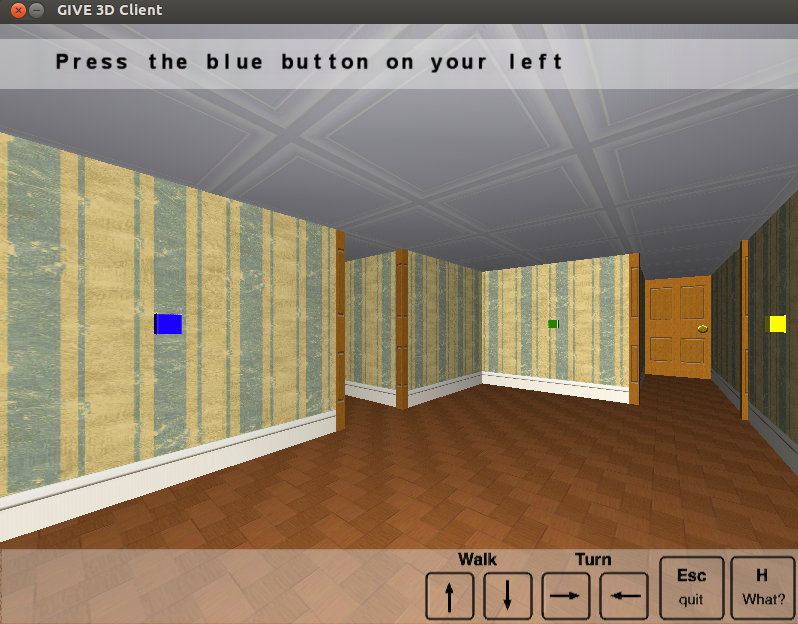
\includegraphics[width=0.7\textwidth]{Images/give-client}
	\caption{A human subject is being navigated through the environment.}
	\label{fig:give-client}
\end{figure}

\citet{koller2010first} state that one of the goals of the GIVE Challenge was spawning interest in NLG, a subfield of computational linguistics (CL), and was inspired by other competitions in the field such as the Recognizing Textual Entailment challenge\footnote{\url{http://pascallin.ecs.soton.ac.uk/Challenges/}} and NIST machine
translation competition\footnote{\url{http://www.itl.nist.gov/iad/mig//tests/mt/}}.

According to \citet{koller2010first}, another important goal was to introduce and explore a new way of evaluating NLG algorithms, techniques and systems in a shared task. More specifically a shared task which was, on the one hand, complex enough to encompass multiple NLG subtasks and, on the other hand, was only concerned with NLG and not any other fields of computational linguistic.

Three basic approaches to evaluation of NLG systems are compared annotated corpora, measuring task performance in an experiment and human judges evaluation. \citet{koller2010first} argue the advantages and disadvantages of these evaluation in more depth, therefore I will only provide a brief summary. The first approach compares output of the NLG system to an annotated corpora, also known as a gold-standard. It is fast and cheap approach, but a problem with it lies in the complexity of the natural language. We can often express concepts in many different ways and there is often no telling which way is a better one. The second approach conducts an experiment and measures task performance on human subjects. Measuring task performance avoids the problems of gold-standard, but it is expensive and time consuming. Lastly, trained human judges are used to evaluate the system. It is less demanding than the second approach, but for the cost of certainty, that the results correspond with results one might achieve with non-expert subjects.

The GIVE Challenge proposes and successfully implements a new, in a sense that it wasn't used for NLG before, approach through Internet-based evaluation. The basic premise is using a client-server software methodology. The client is a program installed on test subject computer, which is easily downloadable from a public website. The client connects through the Internet to a matchmaker server and random evaluation world is selected. Matchmaker also connects the client to a randomly selected NLG system, which itself, can be hosted on a different server. Client and NLG systems then communicate back and forth until the task is finished. Matchmaker finally logs the entire sessions to database. Figure \ref{fig:give-clientserver} shows that architecture in a simple diagram.

\begin{figure}[!htbp]
  \centering
	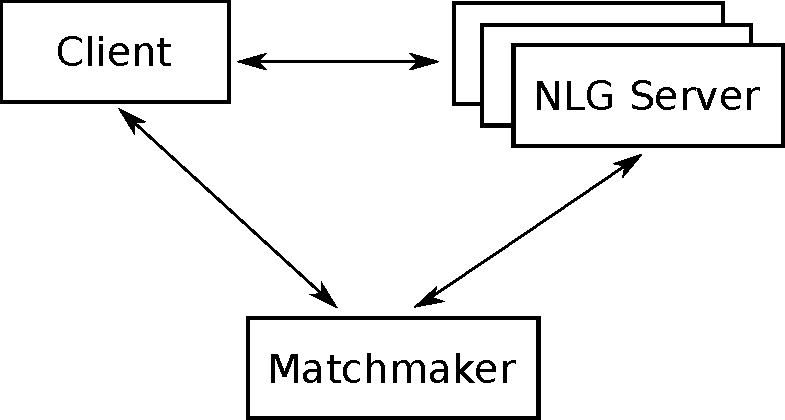
\includegraphics[width=0.7\textwidth]{Images/give-client-servers}
	\caption{Software architecture of GIVE Challenge.}
	\label{fig:give-clientserver}
\end{figure}

This approach immediately presents several advantages. It does not require physical presence of the test subject in a laboratory. The subject simply downloads the client from a website and is able to do the experiment at his/her convenience. Second obvious advantage is a scalability. The number of individuals which can parallelly undertake the experiment is only limited by the servers' load. Thanks to the low costs, advertisement becomes the decisive limitation on the number of subjects. Take for example second instalment of the GIVE Challenge which had up to 1800 participants.

On the other hand, part of the control over the experiment is lost in this approach; for example the control over subject pool. Another problem which rises with this approach is that individuals can repeat the experiment.

In addition to Internet-based evaluation, the GIVE Challenge utilizes variety of evaluation measures of both objective and subjective nature. Among objective measure are task success rate, number of instructions or time required to finish the task. For subjective measures a questionnaire was used at the end of the session. The questionnaire mostly used a 5 point scale with question such as how clear where the instruction or how friendly was the system. Some of the measures intentionally collided with each other, putting emphasize on a certain characteristic of the system.

Having presented the basic concept of the GIVE Challenge and reasons for its creation, I will now move onto brief history of this competition. 

 
\section{History of GIVE Challenge}
The first instalment of GIVE Challenge (GIVE-1) was publicized in March 2008. \citet{koller2010first} report on this instalment and are the source of following information. For more details please refer to their paper. The data collection period was from November 2008 to February 2009. Four teams participated in this challenge, namely from these universities: University of Texas at Austin, Universidad Complutense de Madrid, University of Twente and Union College. The team from University of Twente submitted two systems, making the final number of systems five.

What is important to note about GIVE-1 is a different world representation from the following instalments. GIVE-1 used discrete square grid for player movement. Player was able to rotate only by $90^{\circ}$ and walk forward and backwards by one square of the grid. That had a major impact on the design of NLG systems. Participating teams at least occasionally used this grid in their references (eg. \textit{move forward three steps}). Afterwards organizers realized that the grid and the discrete movement made the task easier than intended and they were after GIVE-1 removed.

Altogether, 1143 valid games were recorded. The demographics featured a majority of males (over 80\%) and wide spread over different countries in the world. For the actual results,  the system from Austin significantly outperformed all other systems in task completion time. At the same time systems from Union and Madrid outperformed other systems in success rate. That shows the significance of different measures for the evaluation. Similar interesting conclusion in both objective and subjective measures can be found in previously mentioned paper. Apart from objective and subjective measures, the report examined influence of English language proficiency and differences between evaluation worlds. The English proficiency had an impact on the task success rate but solely for the least proficient category. The evaluation world also had a significant influence on the task success rate.

Finally, the first instalment also compared the Internet-based evaluation with more standard laboratory evaluation. The conclusion was that Internet-based evaluation provides meaningful results comparable and even more precise in some areas to the laboratory setting.

The second instalment (GIVE-2) run from August 2009 (data collection starting in February 2010) to May 2010 and is thoroughly described by \citet{koller2010report}. Following information are based on this paper. Biggest difference to the GIVE-1, which was mentioned previously, is that players were now able to move freely. This made the instruction generation considerably harder. Additionally, the questionnaire was revised and a few new objectives measures were introduced. Evaluation worlds used in GIVE-2 were considerably harder than in GIVE-1. Number of distracting buttons was increased and same-colored buttons were in some cases next to each other. Also number of alarm tiles was increased. Otherwise, the architecture and the rest of the details stayed the same as in GIVE-1.

This time 1825 games were played over seven NLG systems developed by six teams from: Dublin Institute of Technology, Trinity College Dublin, Universidad Complutense de Madrid, University of Heidelberg, Saarland University and INRIA Grand-Est in Nancy (2 systems).

There was a big drop in success rate, most likely linked to the free movement and the increase of difficulty in the evaluation worlds. Similarly to results in GIVE-1, there was an influence of English proficiency and game world on the task success rate. Additionally, age of the subject played a role in the time required to finish the task and number of actions to finish the task (younger subjects being faster and requiring less actions). The difference between genders in time required to finish the task disappeared in GIVE-2.

Some teams participating in the GIVE Challenge tried to use a corpora of a human to human interactions in GIVE scenario. They were learning language expression or decision-making process and applying them in their NLG systems. The teams were however relying on small self-collected datasets. In a light of this, organizers of GIVE Challenge decided they would collect and provide dataset for future use. \citet{gargett2010give} describe this dataset, which was used in the next instalment of the GIVE challenge.

Following GIVE-2 was so called Second Second instalment (GIVE-2.5), which kept almost the same settings as GIVE-2. There was just a small addition to objective measures and a reduction in the number of subjective questions. The data collection took place between July 2011 and March 2012. \citet{striegnitz2011report} report on the partial results of 536 valid games from July and August 2011, which however constitute a majority of the final number of 650 valid games.

Eight NLG systems participated from 7 teams: University of Aberdeen, University of Bremen, Universidad Nacional de Córdoba, Universidad Nacional de Córdoba and LORIA/CNRS, LORIA/CNRS, University of Potsdam (2 systems) and University of Twente. In this instalment the teams employed more broad spectrum of approaches. Team from University of Bremen used decision trees learned from GIVE-2 corpus. Universidad Nacional de Córdoba and LORIA/CNRS, LORIA/CNRS selected instructions from a corpus of human to human interactions. The teams also often included algorithms from existing NLG and CL literature.

Apart from comparing the systems through objective and subjective measures, \citet{striegnitz2011report} again examined effects of evaluation worlds and demographics factors on task success rate. The evaluation worlds and the English proficiency had an effect. Additionally computer expertise and familiarity with computer games significantly influenced the task performance. The difference between male and female subject wasn't significant.



The following section describes the shared task in more detail and lists possible contents of the GIVE virtual worlds.

\section{Task and GIVE world}
\label{sec:task-give-world}
The GIVE world is a 3D virtual world. The world is an indoor environment, comprising of rooms  connected by doors. It's defined in a human-readable format and stored in a text file. The following objects can be places in a world:

\begin{itemize}
\item
Alarm tile
\item
Button
\item
Door
\item 
Landmark
	\begin{itemize}
	\item
	Bed	
	\item
	Chair	
	\item
	Couch	
	\item
	Dresser
	\item
	Flower	
	\item
	Lamp
	\item
	Table
	\item
	Window
	\end{itemize}
\item
Picture
\item
Safe
\item
Trophy
\item
Wall
\end{itemize}
In addition, some of these objects can have attributes, states or can operate other objects. Buttons have colors as an example of attribute. Doors and safes can be in a closed or an open state. Buttons can operate doors, safes or pictures.

Walls are actually created automatically by defining shapes of rooms. Rooms can have rectangular shape or can be defined by a polygon. I will sometimes use a term ``corridor'' which is a connecting room, usually not containing any button.

The landmarks serve as a decoration but they can be used in an expression generation. Picture is technically a landmark as well, but in GIVE Challenge it often serves another purpose. It covers the safe and needs to be put aside by a button press.

\begin{figure}[!htbp]
  \centering
	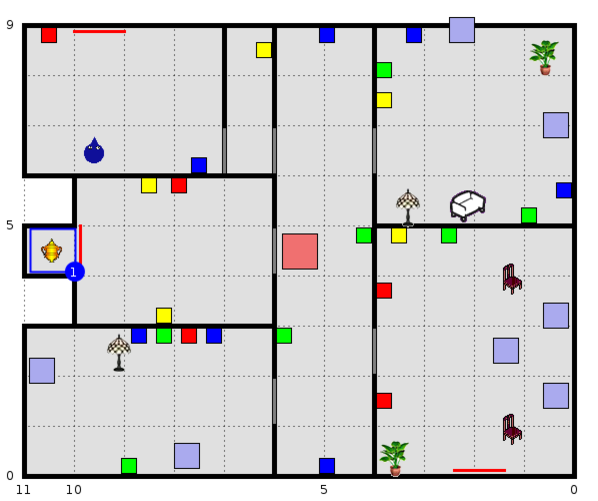
\includegraphics[width=0.75\textwidth]{Images/give-evalworldexmaple}
	\caption{Example GIVE world viewed in GIVE map viewer utility.}
	\label{fig:give-evalworldexmaple}
\end{figure}

Figure \ref{fig:give-evalworldexmaple} shows an evaluation world number one from GIVE-2.5. In top-left room we can see player starting position. Buttons are colored squares on the walls. Grey bars on the walls are closed doors. Trophy in a safe is in the middle-left room. There are also landmarks (like lamp or chair) and one big read square marking an alarm tile.

The flexibility of GIVE world creation allows relatively broad range of scenarios for the task. On the other hand, all the GIVE Challenge instalments consisted of similar sequence of steps.

The goal of all the GIVE Challenge worlds is to pick up a trophy. The trophy is hidden in a closed safe. In order to open the safe a sequence of buttons, usually counting somewhere around 6 buttons, has to be pressed. The safe can be also hidden by a picture, which needs to be put aside. The buttons in a safe-opening series are often in different rooms. Rooms can be also closed off, requiring another button press to open the door. While moving around the world, player has to avoid alarm tiles. Stepping on an activated alarm tile causes an immediate loss. Alarm tiles can also block the path and need to deactivated by a button press. Some buttons also cause an alarm and an immediate loss.

Depending on the number of rooms, complexity of buttons arrangement and length of safe-opening sequence, the task can range from short and trivial problem easily handled by a few instruction templates, to a long and hard case, where it's impossible to capture every possible scenario.

To summarize, navigation system of a player in the GIVE world has to deal with following steps. Note that their order depends on the world definition and they can be thought of as layers of behaviours the system must enforce on player.

\begin{itemize}
\item
Avoid alarm tiles
\item
Avoid pressing alarm-causing buttons
\item
Deactivate path-blocking alarm tiles by a button press
\item
Open closed-off rooms by pressing correct buttons
\item
Press a sequence of buttons to open the safe
\item
Reveal safe behind a picture by pressing correct button
\item
Take the trophy
\end{itemize}

After the safe was opened and possibly revealed from behind the picture player can pick up the trophy and therefore win the game.
\chapter{The S-GIVE Dataset}
\label{chap:s-give}
After GIVE 2.5 instalment presented in Chapter \ref{chap:give-challenge}, Prof. Kristina Striegnitz, Ph.D., one of the organizers of the GIVE Challenge, decided to collect a new dataset of spoken communication, called the S-GIVE Dataset. This chapter serves as an introduction to this dataset.

As a side note, \citet{striegnitz2012referring} report on a smaller German dataset, which is similar to the one I will be talking about. 

The S-GIVE dataset is different from previous GIVE Challenge experiments because the instructions were given by another person and were of a spoken form. In the following chapters, the term Instruction Giver (IG) will be used for the person giving instruction while the navigated person will be called Instruction Follower (IF). Also, let's assume the IG is a female and IF is a male.

The spoken form of instructions changes many aspects of the discourse. For one thing, the IG knows when the IF received her instruction, which is not true for the written instructions. That promotes faster feedback and allows interrupting during an instruction. However, in some cases, the spoken word tends to be less formal and grammatically correct. Moreover, interjections are very common, as are incomplete sentences. That makes the S-GIVE dataset complicated yet interesting to explore.

The data-collection started in July and finished in November of 2012. Through that period 21 interactions between two human subjects were recorded. Originally, 22 pairs participated, but one of the pair failed to finish the tasks and is excluded from the dataset. The subjects were asked to bring someone they know and they were financially compensated for the effort. 

The set-up for the experiment is shown in Figure \ref{fig:give-experiment-setup}. The role of IG, which is on the right in Figure \ref{fig:give-experiment-setup}, was essentially the role of the NLG system in the GIVE Challenge. She was able to see a map of the world, which was updated in real-time and she got information about all necessary steps to finish the task. In addition, she was able to see the other person's client screen. She communicated with the IF through a microphone and her goal was to navigate him through the world and make him finish the treasure-hunt.

\begin{figure}[!htbp]
  \centering
	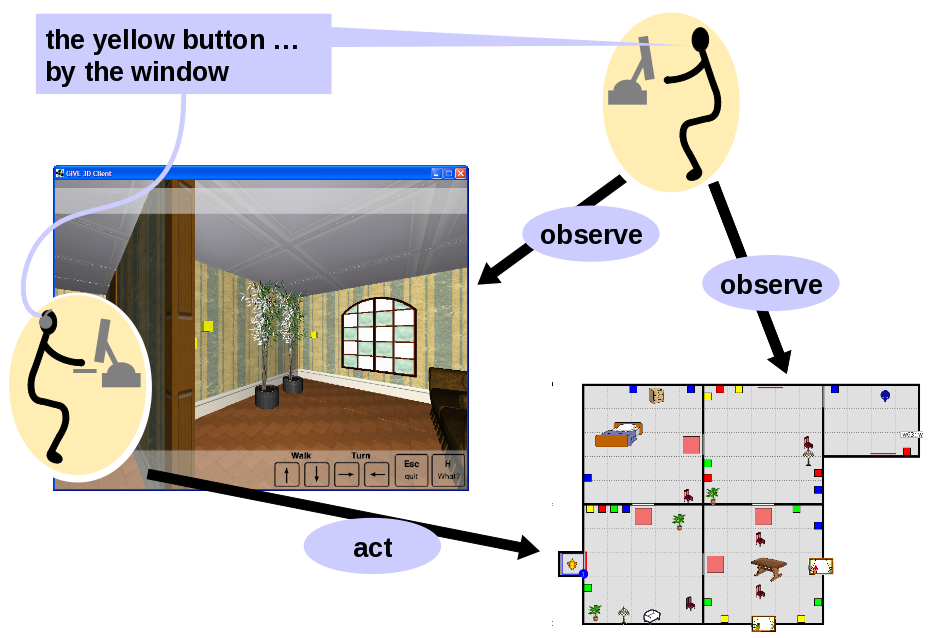
\includegraphics[width=0.7\textwidth]{Images/experiment-set-up}
	\caption{Experiment set-up of data collection}
	\label{fig:give-experiment-setup}
\end{figure}

The IF is on the left in Figure \ref{fig:give-experiment-setup}. He interacted with the client and moved the avatar around the world and was able to press buttons. He listened to the IG's instructions through a headset.

Each pair played one short tutorial world. After that they switched the roles of instruction giver and instruction follower. Following the tutorial was one ``normal'' world randomly chosen from two variants, marked world 1 and world 3 in the dataset. Maps of the worlds 1 and 3 are in Figures \ref{fig:dataset-world1} and \ref{fig:dataset-world3} respectively. Finally they did a difficult version of the other variant (if they started with world 1 the difficult version was for world 3 and vice versa). The difficult versions are marked 1-d and 3-d in the dataset. A difficult version of the world had an increased number of distracting buttons and landmarks compared to the ``normal'' version, as can be seen in the map of world 1-d in figure \ref{fig:dataset-world1d}. If not not stated otherwise, the short tutorial worlds are normally excluded from the analysis.

\begin{figure}[!htbp]
  \centering
	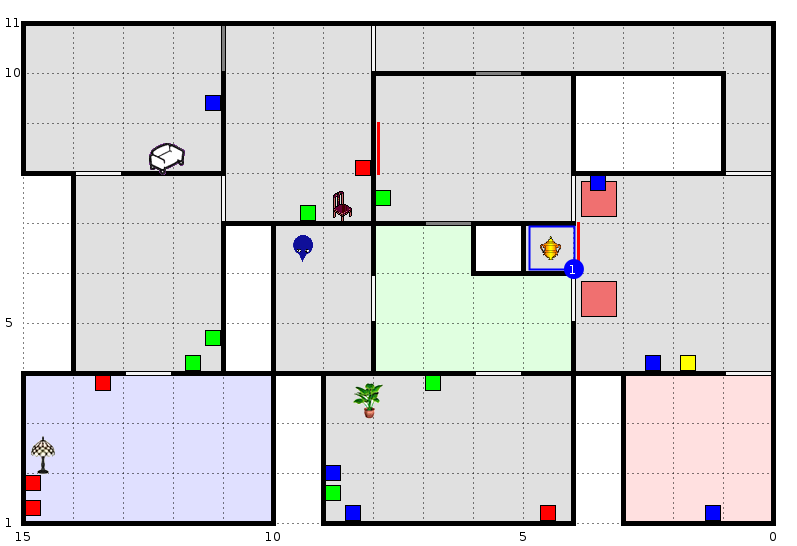
\includegraphics[width=0.7\textwidth]{Images/dataset-world1}
	\caption{Map of the world 1 - normal version.}
	\label{fig:dataset-world1}
\end{figure}

\begin{figure}[!htbp]
  \centering
	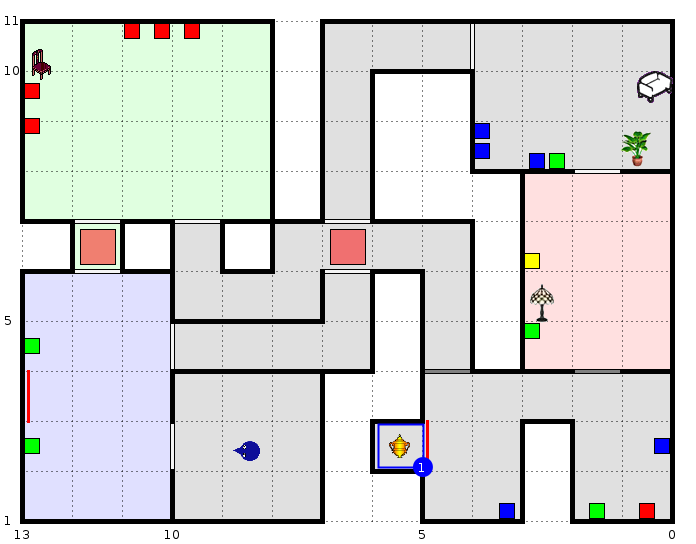
\includegraphics[width=0.7\textwidth]{Images/dataset-world3}
	\caption{Map of the world 3 - normal version.}
	\label{fig:dataset-world3}
\end{figure}

\begin{figure}[!htbp]
  \centering
	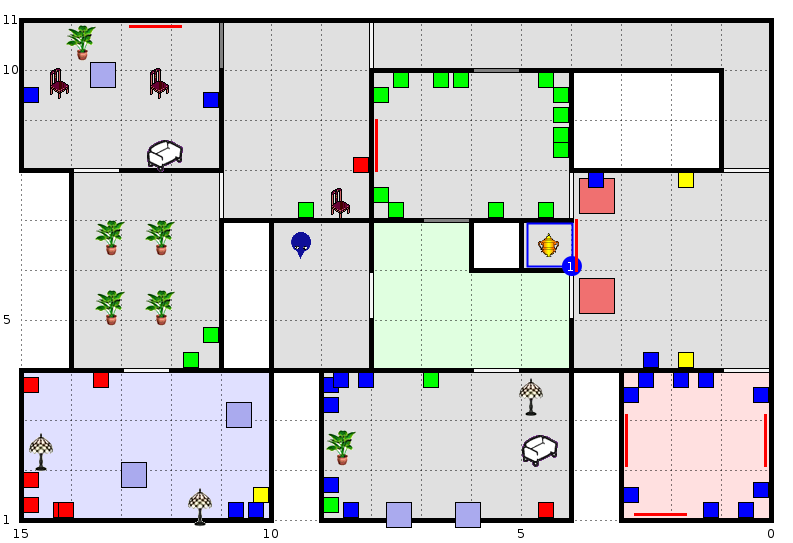
\includegraphics[width=0.7\textwidth]{Images/dataset-world1d}
	\caption{Map of the world 1 - difficult version.}
	\label{fig:dataset-world1d}
\end{figure}

Similarly to the GIVE Challenge, after all 3 rounds subjects were asked to fill in a questionnaire. Its purpose was to get demographic and other relevant information on subjects. The questionnaire can be divided into three parts. The first part was only filled out by the IF and rated the IG and his instruction giving on a scale from 1 to 7. The complete list of the first part questions follows: 

\begin{enumerate}
\item
Overall, my partner gave me good instructions.
\item
Interacting with my partner wasn't annoying at all.
\item
My partner's instructions were clearly worded.
\item
When I had problems with the instructions, we solved them quickly.
\item
I enjoyed solving the task.
\item
I felt I could trust my partner's instructions.
\item
I really wanted to find that trophy.
\item
My partner immediately offered help when I was in trouble.
\item
I would recommend this experiment to a friend.
\item
My partner's instructions were not repetitive.
\end{enumerate}


The second part was filled by both the IF and the IG and was concerned with their navigation skills. To measure the ability to navigate in the world the Santa Barbara Sense of Direction (SBSOD) scores were used \citep{hegarty2002development}. Again the questions were on a scale from 1 to 7. Note that some of the question in the following list are of positive nature (higher rating equals better navigation skill) while other are of negative nature, therefore these scores had to be normalized.

\begin{enumerate}
\item
I am very good at giving directions.
\item
I have a poor memory for where I left things.
\item
I am very good at judging distances.
\item
My "sense of direction" is very good.
I tend to think of my environment in terms of cardinal directions (N, S, E, W).
\item
I very easily get lost in a new city.
\item
I enjoy reading maps.
\item
I have trouble understanding directions.
\item
I am very good at reading maps.
\item
I don't remember routes very well while riding as a passenger in a car.
\item
I don't enjoy giving directions.
\item
It's not important to me to know where I am.
\item
I usually let someone else do the navigational planning for long trips.
\item
I can usually remember a new route after I have travelled it only once.
\item
I don't have a very good "mental map" of my environment.
\end{enumerate}


Finally, the last part of the questionnaire was of a demographic character. We can see questions about age, gender, language and computer expertise, 3D games experience and knowledge of the partner in the following list.

\begin{enumerate}
\item
What is your age?
\item
Are you male of female?
\item
What is your profession / major / favorite subject in school?
\item
How would you rate your computer expertise?
\item
How familiar are you with 3D computer games?
\item
How many hours per week to you play 3D computer games?
\item
Was there a time in your life when you played more 3D computer games? If so, how many hours did you play then?
\item
What languages do you speak? Please indicate how well you speak each on a scale from 1-5, where 5 is your native language.
\item
Did you already know the second participant?
\item
How well do you know the second participant?
\item
Have you worked collaboratively with the second participant before? (For example, when doing homework or preparing a class presentation?)
\item
Have you played 3D computer games with the second participant before?
\end{enumerate}

Many of these questions are explored in the next chapter as potential factors influencing the task performance. 

As was mentioned in Chapter \ref{chap:give-challenge}, the entire session is logged to a database. The player's position, orientation and all visible objects are logged at a fixed rate, approximately every 200 ms. Moreover, other information such as buttons presses or the end of the session are also stored in the logs. Because the worlds are static, distances and angles between the IF and other game objects are easily computed from these logs.

Apart from the logs, there are of course sound files of the IG giving directions. These were transcribed and together with some information from the logs transformed into ELAN files. ELAN is an annotation software \citep{sloetjes2008annotation}. The term \textit{automatic annotations} will be used for the ELAN files created from the logs and transcribed audio in the following text (however note that transcribing audio was done manually). 

These automatic annotations served as a base for creating manual annotations. Manual annotations are primarily concerned with referring expressions and also stored in ELAN format. Most referring expressions in GIVE aim to locate a button, which needs to be pressed. The button, which is a goal of a referring expression, will be called the target button in the following text. Which button is the target button of a reference is one of the layers in the manual annotations. Another layer of the annotations is some basic categorization of the references, whether it is a reference to a single button, to a group of button, to a landmark and so on. The third layer looks deeper into the contents of the reference. It notes whether the reference contains for example the color of a button, whether distractors or landmarks are part of the reference or whether the reference explicitly points out that the button was already pressed before.

The previously mentioned logs, automatic annotations and manual annotations together form the dataset this chapter is dealing with.

An example of an interaction between an IF and an IG is in the following text. Spatial information is transcribed in parentheses for the sake of clearness.

\begin{verse}
(IF enters a room)\\
IG: Go towards the red buttons.\\
(IF turns right and start walking, but he turns too much)\\
IG: No the ones next to the lamp...\\
(IF corrects his direction)\\
IG: Yeah that lamp. On the right.\\
(IF is facing three buttons.)\\
IG: Press the button on the wall you are looking at, that's far from the lamp and on the left. \\
(IF goes towards the correct button and stops close to him)\\
IG: Press it.\\
\end{verse}

After introducing the S-GIVE dataset, the next chapter will contain my analysis of it and machine learning attempts on it.





\chapter{Machine Learning on RE}
RE are big part of language realization of a navigation system and especially so in the GIVE scenario. Part of my work were attempts to apply machine learning techniques on S-GIVE dataset with a clear goal to help navigation system with RE. This part is presented in this chapter.

In the first section I'll describe attempts at predicting timing of the first reference to a target button. Second section talks about modeling of chains of references. Third section briefly touches a topic of using room memory. In the last section, I will present my thoughts on the results of previous sections.

\section{Timing of the first reference}
\label{sec:timing-firsref-ml}
Work of \citet{stoia2006sentence} was previously mentioned in related work section of chapter \ref{chap:bg}. They applied machine learning on timing of the first reference in a 3D virtual world. The set-up of their experiment is quite similar to the GIVE's one and so I decided it would be interesting to replicate their methodology on GIVE dataset. 

I defined the problem of the timing of the first reference as a classification task, as did \citet{stoia2006sentence}. More precisely binary classification, the two classes being either refer to the target button or delaying the reference. After extracting the first references to buttons which needed to be pressed from the dataset, I excluded plural references, because of their complexity. Some buttons were placed on top of each other and IG wasn't sure which one need to be pressed. These were excluded as well because of the unnecessary confusion. That left me with 351 first references. For each first reference I have chosen one negative example, where IG could refer to the target but chose not to. I picked negative examples randomly from interval between entering room and time of the first reference. Overall, that is 702 data-points with perfectly balanced classes.

As for features extraction, I have chosen similarly to \citet{stoia2006sentence} various spatial information. For the positive examples, I averaged these spatial information over 0.6 seconds window centered on the time of the reference. Reasoning for that, is that IG take scene situation into consideration before and possibly after they start uttering the reference. For negative examples I chose not to averaged them, since they are chosen randomly. All features are listed in the following list. The list also includes figures' numbers. These figures are histograms of the attributes, separated for both classes and can be found in appendix.

\begin{itemize}
\item
Distance to target button - Figure \ref{fig:fref-distrib-dist}
\item
Absolute value of angle to target - Figure \ref{fig:fref-distrib-angle}
\item
Whether target is visible (True/False) - Figure \ref{fig:fref-distrib-visib}
\item
Number of distractors - Figure \ref{fig:fref-distrib-distractors}
\item
Number of distracting buttons - Figure \ref{fig:fref-distrib-distbuttons}
\item
Number of visible buttons with smaller angle to IF than the target button - Figure \ref{fig:fref-distrib-distangles}
\end{itemize}

Once I have extracted these features I used three machine learning techniques: C4.5 decision tree because of their easy interpretation, naive Bayes to observe effect of all attributes and Support vector machine for linear classification. I used Weka software implementation of previous algorithms \citep{hall2009weka}.

For all the algorithms I used a standard ten-fold cross validation. The results can be seen in table \ref{tab:firstref}. Pruned decision tree for timing of the first reference can be seen in figure \ref{fig:dectree}. I used two simple baselines to compare the results with. I have perfectly balanced classes so the first baseline is 50\%. Simple rule for the first reference is to refer when the target is visible, and delay it if the target is not visible. In my case that rule has an accuracy of 64.2\%. 

\begin{table}[!htbp]
 \centering
\begin{tabular}{lr}
\toprule
Model    & Accuracy (\%)  \\
\midrule
Class baseline    & 50.00\\
Visibility baseline & 64.2\\
\midrule
Naive Bayes  & \textbf{64.70} \\
C4.5 & 63.31 \\
SVM & 55.42 \\
\bottomrule
\end{tabular}
\caption{Results of first reference timing modeling}
\label{tab:firstref}
\end{table}

Only one algorithm was able to get over visibility baseline and not by a significant amount. These results were surprising, because \citet{stoia2006sentence} had success with the same approach on a similar dataset. Reasons for this difference are probably in the differences between their experiment and GIVE set-up. First, their tasks also included different actions than pushing buttons (e.g. picking up items). Second, their worlds had higher diversity of the distractors and smaller frequency of them. With increasing number of distractors and particularly distractors of the same category, it seems that spatial features loose their power in predicting the timing of the first reference. The number of visible distractors was the best attribute in their decision tree, but in my tree (figure \ref{fig:dectree}) it had lower information gain. Moreover, the decision tree did the split on the number of visible buttons not the number of all visible distractors.

After the timing of the first references classification proved to be more difficult than excepted, I have switched from predicting the timing of the references to predicting their content. Next, I focused on chains of references.

\begin{figure}[!htbp]
 \centering
\small
\begin{verbatim}
Distance to target <= 4.45
| Is target visible? = False: DELAY
| Is target visible? = True
| | Distance to target <= 2.51: REFER
| | Distance to target > 2.51
| | | Number of distracting buttons <= 4.67: REFER
| | | Number of distracting buttons > 4.67: DELAY
Distance to target > 4.45: DELAY
\end{verbatim}
\caption{Decision tree for first reference timing}
\label{fig:dectree}
\end{figure}

\section{Chains of references}
Section \ref{sec:dataset-chains} introduced the phenomenon of chains of references. It also analysed various linguistic functions, the chains can play in REG. This section will build on top of this analysis, by employing machine learning techniques to model the chains.

Valid and important question is whether chains aren't something, which should actually be avoided, instead of modelled. That is, what is the relation between usage of chains and task performance measure, such as duration. To address this issues, I used linear regression predicting the duration of the experiment explained by the average chain length. Figure \ref{fig:chains_dur_scatter} does contain a hint of a trend, but also contains a lot of counter-examples. 

\begin{figure}[!htbp]
  \centering
	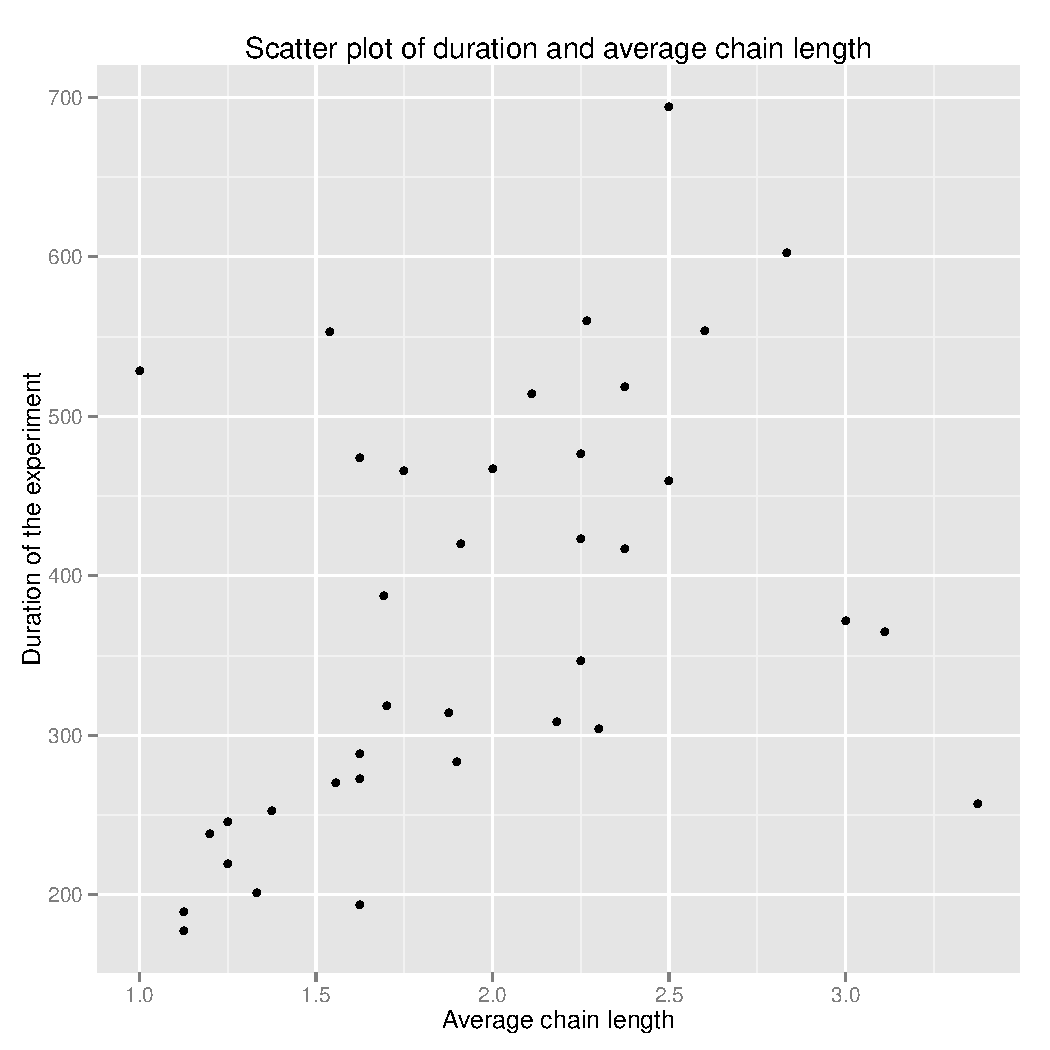
\includegraphics[width=0.8\textwidth]{Images/chains_duration_LR}
	\caption{Scatter plot of duration and chain length}
	\label{fig:chains_dur_scatter}
\end{figure}

When I applied linear regression the $R^2$ was 0.188, which means the average chain length explains very little of the duration variation. If the average chain length was to significantly influence the duration, I would except much higher $R^2$. Correlation between the duration and average chain length is not low: 0.433, however correlation does not imply causation. Longer chains can be caused by errors of IF or IG and the errors are also likely to increase the duration. Based on these facts, I don't believe the chains are harmful phenomenon and it makes sense to proceed with attempting to model them. 

With modeling the chains of references, there are numerous problems to tackle. Simple presence of the chain can be thought of as a classification task. It can be interesting try to predict the chain length. Having established common linguistic functions of the chains, classify chains whether they would contain these function is another task to consider. I looked into each of these problem and together with extracting relevant features, thoroughly explored using machine learning for modeling the chains.

As a side note, during exploring chains of references I switched from Weka implementation of machine learning techniques \citep{hall2009weka} to scikit learn package for Python \citep{scikit-learn}. The main reason being easier automation of the entire pipeline, therefore speeding-up of the whole process and more control over whole process.

\subsection{Presence of the chains}
From Section \ref{sec:dataset-chains}, the functions the chains can play in a discourse are known. However, what role does play the scene complexity and particular situations in the presence of the chains? Will more complex scene spawn more chains or are the chains too complex to be captured by simply looking at where they are created? To answer these question, I extracted scene complexity features and the target button for all references and classified whether the chains was present or not.

The features I extracted from the dataset are in the following list:

\begin{itemize}
\item
Target button	
\item
Number of objects In the room - Figure \label{fig:chains-distrib-objects}
\item
Number of buttons in the room - Figure \label{fig:chains-distrib-buttons}
\item
Number of landmarks in the room - Figure \label{fig:chains-distrib-landmarks}
\item
Number of very close buttons to the target button (closer than 0.3m) - Figure \label{fig:chains-distrib-veryclose}
\item
Number of buttons on the same wall as target button - Figure \label{fig:chains-distrib-samewall}
\item
Number of close buttons to the target button (closer than 1m) - Figure \label{fig:chains-distrib-close}
\item
Number of far buttons (farther than 1.5m) - Figure \label{fig:chains-distrib-far}
\end{itemize}

The target button is a categorical feature, so I used DictVectorizer class in scikit to transform it into multiple numerical features. I further tried to use all features, select 8 best features using SelectKBest class from scikit with $\chi^2$ statistic as a scoring function and select 16 best features using the same strategy. For algorithms I used Decision Tree, Naive Bayes, Support Vector Machines (SVM), One-Nearest Neighbour (1-NN), Two-Nearest Neighbours (2-NN) and Random Forest. This selection employs various approaches for classification task, each of the algorithms having strong and weak points. For evaluation, I used standard ten-fold cross validation and compared the accuracy of the classifiers with majority class baseline. From now on, I will also include double the standard deviation (std). The idea behind the double is that if the features follow normal distribution and the three sigma rule is applied, the chance of the accuracy being in interval of $\pm$ standard deviation times two is 95.45\% . The results are summarized in Table \ref{tab:chains-ml-presence}. 

\begin{table}[!htbp]
 \centering
\begin{tabular}{lccc}
\toprule
Features & Model    & Mean accuracy (\%) & $2\times$ Std \\
\midrule
Majority baseline &    & 55.2	& \\
\midrule
All & Decision Tree 	& 55.5		& 13.5 	\\
	& Naive Bayes  	& 55.8		& 6.6 	\\
	& SVM 			& 56.1		& 11.2 	\\
	& 1-NN			& 56.3		& 9.3 	\\
	& 2-NN			& 53.6		& 12.1 	\\
	& Random Forest	& 55.0		& 13.6	\\
\midrule
8 best 	& Decision Tree 	& 	59.7		& 14.6  	\\
		& Naive Bayes  	&	56.4		& 2.9 	\\
		& SVM 			&	58.3		& 13.1 	\\
		& 1-NN			&	58.8		& 11.1 	\\
		& 2-NN			&	56.1		& 14.4 	\\
		& \textbf{Random Forest}	&	\textbf{60.0	}	& 16.6 	\\
\midrule
16 best & Decision Tree 	& 55.8	& 13.5  	\\
	& Naive Bayes  		& 56.4	& 2.9 	\\
	& SVM 				& 58.3	& 13.9  	\\
	& 1-NN				& 56.9	& 9.1  	\\
	& 2-NN				& 53.3	& 12.8  	\\
	& Random Forest		& 57.2	& 12.8  	\\	
\bottomrule
\end{tabular}
\caption{Results of chains presence modeling}
\label{tab:chains-ml-presence}
\end{table}

The best mean accuracy had the Random Forest for 8. However, it wasn't significantly better than majority class baseline. Take into account the standard deviation, none of the classifier and features combination outperformed the baseline.  From these results, I conclude that the chains presence is not dependent only on the scene complexity and specific scenarios. IG strategies for referencing, IF behaviour and other circumstances play role in creation of the chains.

\subsection{Chain length prediction}
After not being able to predict presence of the chains based on spatial information and target button, I was interested if I could predict the chain length based. I used same attributes as in previous classification of the chains' presence, but added two more features concerned with IF movement behaviour. Namely, the ratio of the time IF spent not moving at all through the chain duration and ratio of the time IF spent only rotating in place through the chain duration. The idea behind these features is that IF who is not moving or just looking around is an indication of him/her being confused, which then should produce more referring expression for the chain.

For reference, I list all features and add figures numbers for the two new attributes:
\begin{itemize}
\item
Target button	
\item
Number of objects In the room
\item
Number of buttons in the room
\item
Number of landmarks in the room
\item
Number of very close buttons to the target button (closer than 0.3m)
\item
Number of buttons on the same wall as target button
\item
Number of close buttons to the target button (closer than 1m)
\item
Number of far buttons (farther than 1.5m)
\item
Ratio of time IF spent not moving - Figure \label{fig:chains-distrib-stop}
\item
Ratio of time IF spent rotating - Figure \label{fig:chains-distrib-rotate}
\end{itemize}

I applied linear regression, predicting chain length based on three groups of mentioned attributes - target, spatial features and IF movement behaviour features. I evaluated the regressions by looking at $R^2$. The results are in Table \ref{tab:chains-lr-length}.

\begin{table}[!htbp]
 \centering
\begin{tabular}{lc}
\toprule
Features & $R^2$  \\
\midrule
Target button & 0.154\\
Spatial & 0.146 \\
IF movement & 0.126 \\
Spatial ad IF movement & 0.262 \\
\bottomrule
\end{tabular}
\caption{Results of chains length modeling}
\label{tab:chains-lr-length}
\end{table}

None of the regressions from Table \ref{tab:chains-lr-length} are particularly good at predicting chain length. Combining spatial and IF movement features does increase the percentage of chain length variation explained by the model, suggesting that these features have, however small, effect on the chain length. Once again it shows that chains are complex phenomenon, influenced by IF, IG and scene variables.

\subsection{Closer look at chains' content}
Despite not being able to predict the chains presence and length, I was still interested in chains and decided to look closely into chains content. First, I took advantage of having annotated the functions in the chains, as introduced in Section \ref{sec:dataset-chains}. I focused on specification and group function and tried to predict whether the chain will contain these functions. Second, I tried to predict whether the chain provide new information about the target button after its first reference. For example IG could add RE about position of the target button relative to a landmark in the third reference of the chain. Reasoning behind this classification is trying to predict when IG add information to the chains.

For all these classification task, I used the same features as in the chain length prediction, that is: the target button, spatial features, IF movement behaviour features and combination of the previous two. Again, I used ten-fold cross validation for evaluation and compared that to majority class baseline. The results for specification function are in Table \ref{tab:chains-ml-specification}, for group function in Table \ref{tab:chains-ml-group} and for predicting new information in Table \ref{tab:chains-ml-infgain}. For algorithms, I maintained broad range of algorithms, similarly to previous machine learning attempts.

\begin{table}[!htbp]
 \centering
\begin{tabular}{lccc}
\toprule
Features & Model    & Mean accuracy (\%) & $2\times$ Std (\%) \\
\midrule
 Majority baseline &   & 74.7	& \\
\midrule
Target button 	& Decision Tree 	& 73.3		& 6.0 	\\
				& Naive Bayes  	& 38.0		& 22.4	\\
				& SVM 			& 74.7		& 5.3 	\\
				& 1-NN			& 70.7		& 14.8 	\\
				& Random Forest	& 74.0		& 7.2	\\
\midrule
IF movement	& Decision Tree 	& 	64.0	& 21.7 \\
			& Naive Bayes  	&	72.7	& 11.1	\\
			& SVM 			&	74.7	& 5.3 	\\
			& \textbf{1-NN}			&	\textbf{77.3	} & 12.2 	\\
			& Random Forest	&	71.3	& 16.9 	\\
		
\midrule
Spatial	 	& Decision Tree 	& 74.7	& 16.7 \\
			& Naive Bayes  	& 66.7 	& 20.7	\\
			& SVM 			& 71.3	& 14.7 	\\
			& 1-NN			& 68.7	& 23.9 \\
			& Random Forest	& 74.7	& 18.7 \\	
\midrule
Spatial and movement& Decision Tree 	& 66.7	& 23.1 \\
					& Naive Bayes  	& 66.7	& 20.7	\\
					& SVM 			& 71.3	& 18.9 	\\
					& 1-NN			& 76.7	& 8.9 \\
					& Random Forest	& 68.0	& 16.7 \\			
\bottomrule
\end{tabular}
\caption{Results of specification function in chains modeling}
\label{tab:chains-ml-specification}
\end{table}

\begin{table}[!htbp]
 \centering
\begin{tabular}{lccc}
\toprule
Features & Model    & Mean accuracy (\%) & $2\times$ Std (\%) \\
\midrule
Majority baseline &   & 75.4	& \\
\midrule
Target button 	& Decision Tree 	& 81.3		& 14.4 	\\
				& Naive Bayes  	& 38.0		& 14.7	\\
				& SVM 			& 75.3		& 6.1 	\\
				& 1-NN			& 79.3		& 13.9 	\\
				& Random Forest	& 79.3		& 17.3	\\
\midrule
IF movement	& Decision Tree 	& 	61.3	& 23.7 \\
			& Naive Bayes  	&	75.3	& 6.1	\\
			& SVM 			&	75.3	& 6.1 	\\
			& 1-NN			&	73.3	 & 15.8 	\\
			& Random Forest	&	68.0	& 16.7 	\\
\midrule
Spatial	 	& Decision Tree 	& 80.0	& 10.3 \\
			& Naive Bayes  	& 77.3 	& 18.1	\\
			& SVM 			& 77.3	& 8.8 	\\
			& 1-NN			& 77.3	& 13.6 \\
			& \textbf{Random Forest}	& \textbf{82.0}	& 13.4 \\	

\midrule
Spatial and movement& Decision Tree 	& 71.3	& 16.9 \\
					& Naive Bayes  	& 78.0	& 15.8	\\
					& SVM 			& 77.3	& 8.8 	\\
					& 1-NN			& 79.3	& 9.3 \\
					& Random Forest	& 74.0	& 18.3 \\	 	
\bottomrule
\end{tabular}
\caption{Results of group function in chains modeling}
\label{tab:chains-ml-group}
\end{table}

\begin{table}[!htbp]
 \centering
\begin{tabular}{lccc}
\toprule
Features & Model    & Mean accuracy (\%) &  $2\times$ Std (\%) \\
\midrule
 Majority baseline  &   & 67.3	& \\
\midrule
Target button 	& Decision Tree 	& 68.3	& 19.6 	\\
				& Naive Bayes  	& 38.0	& 15.8	\\
				& SVM 			& 67.3	& 4.0 	\\
				& 1-NN			& 56.0	& 31.1 	\\
				& Random Forest	& 68.0	& 19.6	\\
\midrule
IF movement	& Decision Tree 	& 	58.7	& 8.0 \\
			& Naive Bayes  	&	68.0	& 11.6	\\
			& SVM 			&	67.3	& 4.0 	\\
			& 1-NN			&	41.3	& 20.5 	\\
			& Random Forest	&	57.3& 12.2 	\\
			
\midrule
Spatial	 	& Decision Tree 	& 68.0	& 16.7 \\
			& Naive Bayes  	& 60.7 	& 28.3	\\
			& SVM 			& 71.3	& 8.5 	\\
			& 1-NN			& 59.3	& 21.9 \\
			& Random Forest	& 67.3	& 17.3 \\	

\midrule
Spatial and movement& Decision Tree 	& 66.0	& 26.3 \\
					& Naive Bayes  	& 62.7	& 26.1	\\
					& \textbf{SVM} 	& \textbf{72.7}	& 9.3 	\\
					& 1-NN			& 59.3	& 19.3 \\
					& Random Forest	& 64.7	& 18.9 \\	 	
\bottomrule
\end{tabular}
\caption{Results of new information in chains modeling}
\label{tab:chains-ml-infgain}
\end{table}

The best classifiers for these 3 tasks can be found in respective results tables, marked by bold font. Similarly to previous attempts, all combinations of attributes and algorithms had the accuracy around the baseline. The last section of this chapter will address these and all previous results to more depth.

\section{Room memory}
Last machine learning problem I tackled was using memory of the previously visited rooms in RE for room switching. When IF has to return to a recently visited room, IG sometimes employ RE such as: ``Go to the room you were just in.'' Deciding whether to use the memory in room switching RE can be thought of as a classification task.

I extracted all moments where IF went between rooms and determined whether the room memory was used from what was IG saying before going into the new room. I also extracted 3 features:

\begin{itemize}
\item
Was IF in the new room before?
\item
How many seconds before, he/she was there?
\item
How many rooms before, he/she was there?
\end{itemize}

The last feature being of a categorical character, once again DictVectorizer was used for transformation and from the transformed numerical values I selected 3 best with SelectKBest and $\chi^2$ statistic. The results are in Table \ref{tab:history-ml}.

\begin{table}[!htbp]
 \centering
\begin{tabular}{lcc}
\toprule
Model    & Mean accuracy (\%) & $2\times$ Std (\%) \\
\midrule
 Majority baseline    & 78.5	& \\
\midrule
 Decision Tree 	& 78.0	& 7.1 	\\
 Naive Bayes  	& 68.3	& 7.3	\\
 SVM 			& 82.2	& 6.2 	\\
 1-NN			& 80.8	& 6.6 	\\
 \textbf{Random Forest}	& \textbf{84.4}	& 6.6	\\
\bottomrule
\end{tabular}
\caption{Results of room memory modeling}
\label{tab:history-ml}
\end{table}

Despite not being able to significantly outperform the baseline using machine learning, I used the knowledge gained in the room memory modeling attempt. In the systems I developed for the experiment, which will be discussed in the last chapter, I created a simple rule for using room memory and enhanced the REG process.

\section{Thoughts on ML in S-GIVE dataset}
Thanks to better availability of annotated corpora, machine learning techniques are becoming popular in the field of REG, examples being mentioned in Section \ref{sec:relwork}. Inspired by similar research, I looked into a S-GIVE dataset, so far unexplored using ML, a dataset of spoken instruction giving in 3D virtual environment.

Despite extensive feature extraction and tackling various problems, the results were unsatisfactory. In this section, I would like to present my thoughts, why I believe that was the case.

First point to explore is the complexity of S-GIVE scenario. As was already discussed in Section \ref{sec:timing-firsref-ml}, S-GIVE worlds have specific properties, which most likely have significant influence on the way IG formulate their instructions. S-GIVE dataset is specific in high frequency of distractors, especially of the same category as the target of the references. To identify targets in such environment often requires taking into account relations between entities. This was one of the original constrains of early REG research, as mentioned in Section \ref{sec:bg-reg}, and only recently this constraint was attempted to be lifted. In some scenarios, the buttons were intentionally organized in complex arrays, where even IG wasn't sure which button needs to be pressed. Spatial features, which proved to be effective in research of \citet{stoia2006sentence}, likely loose their predictive power when dealing with situations of frequent distractors of the same type as the target.

The dataset size have to be taken into account, when discussing the ML results. The relatively small number of participants and, on the other hand, higher number of scenarios, where REs were created, is something to consider. With smaller number of participants, IGs' personal strategies of referencing will play bigger role in the analysis. Some might prefer to reference the target button immediately, while others might postpone the reference until they removed more distractors through other movement instructions. These difference obviously make any attempts of machine learning difficult on a small dataset. With enough data it would be possible to separate strategies to clusters and examine each clusters separately. However with 20 participants, this is not possible or very difficult to achieve. These strategies are also likely to be influenced by IFs, further increasing uniqueness of REs produced for each pair of IG and IF. I strongly believe bigger dataset would be more successful in applying ML techniques.

Last but not least, there is a question of used features. Spatial features are easier to extract from S-GIVE dataset than any other. While I attempted using other features apart from the spatial ones, they extraction is problematic and time consuming. I would speculate that the features about IF's behaviour and IG's personality might increase accuracy of presented models, but exploring them was beyond scope of this thesis. Not to mention, that some interesting features of a more personal character don't necessarily have to be in dataset at all and one would have to repeat the experiment to collect them.

That being said, the ML attempts inspired in many ways the systems I used in the experiment in following chapter. 





\chapter{Experiment on RE}
Throughout this thesis, I was interested in a strategy of referring, where the first reference does not always uniquely identify the target object. Instead, the strategy relied on a feedback and additional references, which together with the first reference formed a chain of references. I wondered what is the effect of this splitting of the information across more references. In Chapter \ref{chap:ml} this strategy was explored through phenomenon of chains of references. After not being able to model this behaviour through methods of machine learning, I decided to look at that strategy under the more controlled conditions of an experiment.

In the first section, I'll present my hypothesis concerning the strategy of splitting references. 

The second section will describe the experimental set-up. 

In the last section, I'll summarize the results of the experiment.

\section{Hypothesis}
To evaluate the strategy of splitting references, I compared two NLG systems, which I have built to resemble human IGs from the S-GIVE dataset. The two systems are identical, except for a difference in the REG strategy for the target button. One system represents the strategy of splitting references, while the other one would represent a more standard approach of referencing. They will be thoroughly described in Section \ref{sec:exper-setup}.

A question this chapter tries to answer is how splitting references affects the task proficiency. Is this strategy significantly different from the more standard fully-identifying references? Or is it simply a language device the IG can utilize in complicated virtual worlds.

I've formulated my prediction to these questions as hypothesis:

\begin{hypo}
Distributing information to uniquely identify the referent across multiple referring expressions separated by non-negligible time intervals does not have an impact on the task proficiency.
\end{hypo}

%\begin{alterhypo}
%Distributing information to uniquely identify the referent across multiple referring %expressions separated by non-negligible time intervals does not have an impact on the %task proficiency.
%\end{alterhypo}

Measuring task proficiency can be done in several ways. In the previous chapters, I've often employed the duration of the experiment. However, for this experiment I've chosen a more specific measure, in order to diminish effects of other factors. I've measured the time from the point of uttering the first reference up to the pressing of the targeted button. This not only diminishes effects of other variables in the navigation process, but can also be interpreted as a measure how well the references were understood by the IF.

For testing the hypothesis I've compared average times between the first reference and the pressing of the target button for both systems. I have used the independent two-sample t-test for unequal sample size. The unequal sample size comes from the fact that a subject could press a wrong button and therefore the number of potential references may vary.

Having formulated hypothesis and translating it into a statistical test, I can now describe how I approached setting up the experiment.

\section{Experimental set-up}
\label{sec:exper-setup}
I've tested my hypothesis through a human subjects evaluation. Each subject did 5 virtual worlds from the GIVE scenario. One of the worlds was a short tutorial world. This tutorial world was excluded from the analysis and served the purpose of diminishing the effect of learning. After the tutorial world, the subjects did 4 evaluation worlds in a random order. The two tested NLG systems were assigned to each world semi-randomly to ensure both of the systems appeared twice. Please note, that the tutorial world was created in such way that the two tested NLG systems behaved the same way and therefore none of the systems had an advantage in number of trials. I've used text instruction presented on the screen as in the GIVE Challenge instalments. Using some sort of speech synthesis or even recorded instructions was beyond the scope of this thesis.

The worlds were similar to the GIVE challenge worlds. Maps generated by the GIVE map-viewer for all of the 4 evaluation worlds can be found in Figures \ref{fig:exper-world1}, \ref{fig:exper-world2}, \ref{fig:exper-world3} and \ref{fig:exper-world4}. I did not include any alarm tiles or alarm-causing buttons in the worlds, to avoid situations where the IF would loose. I also avoided complex arrays of buttons, which were present in some of the S-GIVE worlds.

\begin{figure}[!htbp]
  \centering
	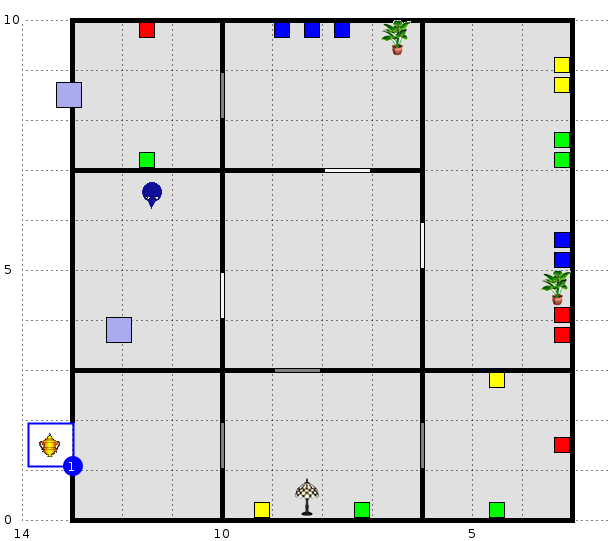
\includegraphics[width=0.7\textwidth]{Images/experiment-world-2}
	\caption{Map of the evaluation world 1.}
	\label{fig:exper-world1}
\end{figure}

\begin{figure}[!htbp]
  \centering
	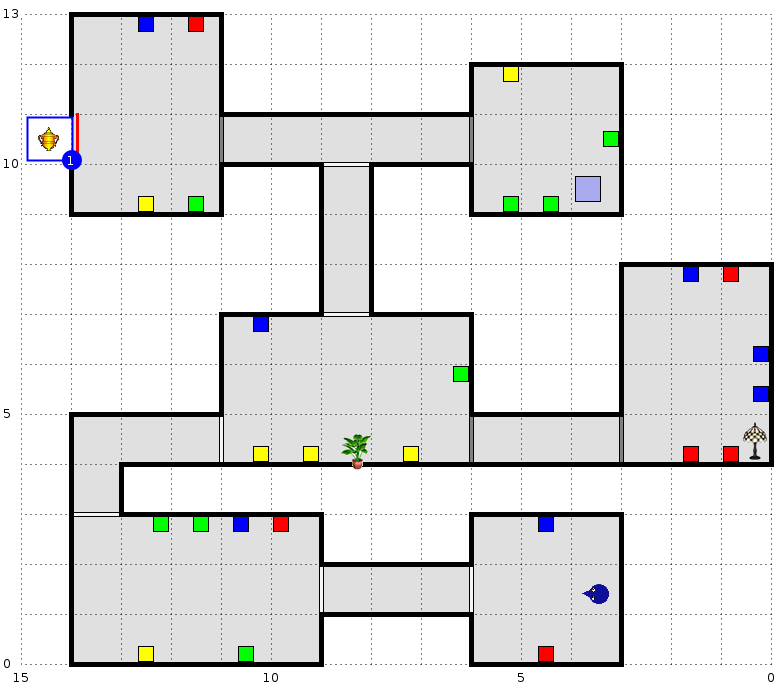
\includegraphics[width=0.7\textwidth]{Images/experiment-world-3}
	\caption{Map of the evaluation world 2.}
	\label{fig:exper-world2}
\end{figure}

\begin{figure}[!htbp]
  \centering
	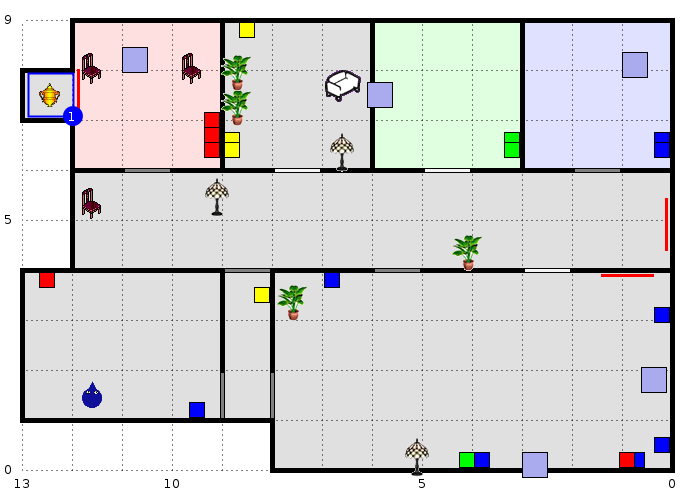
\includegraphics[width=0.7\textwidth]{Images/experiment-world-4}
	\caption{Map of the evaluation world 3.}
	\label{fig:exper-world3}
\end{figure}

\begin{figure}[!htbp]
  \centering
	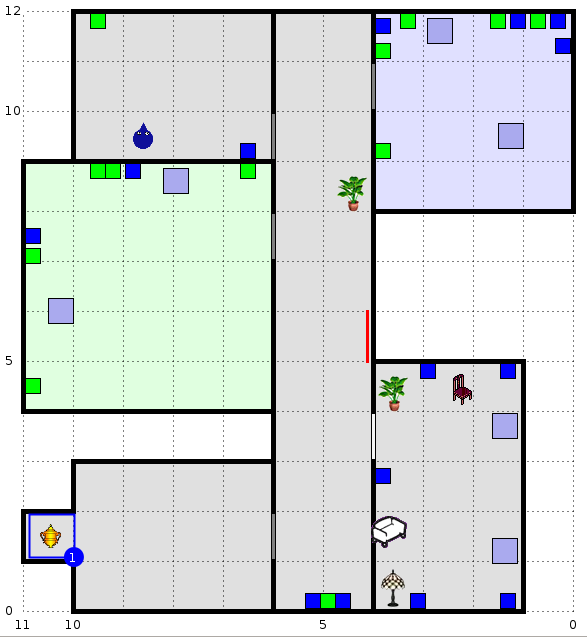
\includegraphics[width=0.7\textwidth]{Images/experiment-world-5}
	\caption{Map of the evaluation world 4.}
	\label{fig:exper-world4}
\end{figure}

I have called the two NLG systems Alpha and Beta. Since they are almost identical except for a REG strategy for the buttons, I will describe the Alpha system and simply point out the differences between it and the Beta system, at the end of the description. As was previously mentioned in Chapter \ref{chap:ml}, the NLG systems are inspired by the analysis of the S-GIVE dataset. Even though the S-GIVE dataset is spoken, I managed to transform some ideas from the spoken data to the written instructions.

Because the final systems are not the subjects of this thesis, but merely a device to examine a NLP phenomenon, I will stick to a high-level descriptions of the ideas behind them and avoid exhaustive software engineering description, such as class diagrams and similar devices.

First thing I would like to address is the timing. In the spoken S-GIVE scenario the IG knows when the IF heard the RE. That is however unknown for the written instruction giving. I have partially solved this problem by estimating the timing with an average reading speed of 150 words per minute. This can of course affect the task proficiency because of personal differences in the reading speed and effects of learning, but it is not easily solved completely in the framework I was using.

For the direction giving, the Alpha system uses 4 directions. The were heavily used in the S-GIVE dataset even though sometimes enhanced by adjectives. The directions are simple: in front of the IF, left, right and behind the IF; all from the IF's point of view. In conjunction with REs which use relations between the world's entities, these 4 directions are sufficient to describe the path for the IF. Suppose we consider $0^{\circ}$ a direction the IF is facing, then I've chosen the limits for the 4 directions as follows: in front $\langle-35^{\circ},35^{\circ}\rangle$, right $(35^{\circ},145^{\circ})$, behind $\langle145^{\circ},-145^{\circ}\rangle$ and left $(-145^{\circ},-35^{\circ})$. The system uses them as in the following example: ``Press the green button on your left.''

Before focusing on RE to the target button, I will report on how I implemented navigating through the rooms. In relatively simple scenarios with rooms and mainly straight corridors, the system can simply create a RE for the door leading to the next planned room, once the IF entered a new room. Adding verbs of movement such as ``go'' to this RE is a simple, yet in the S-GIVE dataset common method for navigating in GIVE scenario. An example of such a sentence is: ``Go through the door in front of you.'' The only complication is that with only 4 directions, other doors can be present in the same direction as the target door. I've solved this by another RE, identifying the target door using its relative position in the group of distracting doors: ``The door closest to you.'' Whenever this specification is needed, I've also added positive feedback when the IF is heading towards the correct doors and negative feedback if he/she enters a wrong room. I have also enhanced this subsystem by two additional improvements commonly seen in the S-GIVE dataset.

First, when the IF is only passing through the room on his way to a next one, I modified the language realization to take advantage of that fact. The system will produce expressions such as: ``Make a left.'' or ``Keep going straight.'' This adds variability to the NLG system and makes it more human-like.

Second, I exploited the room memory, first presented in Section \ref{sec:room-memory-ml}. When the IF is immediately returning to the room he/she was just in and the time elapsed since he/she was there is not large (less than 20 seconds), the system will produce an expression such as: ``Go back to the room you were just in.'' This addition not only increase human-likeness, but I would argue also has an impact on the task efficiency, since it avoids a lot of problems in the standard method described above.

The most complicated task are REs to a target button. This is where the systems Alpha and Beta differ. Once the IF enters the room where a button needs to be pressed, the systems decide whether a reference containing the color of the button and the direction to the button will uniquely identifies the target button. That is, whether there are distracting buttons of the same color in the same direction. If there are none, both systems simply generate a RE like this one: ``Press the green button behind you.'' However, if this (first) RE would not uniquely identify the button, additional information must be provided. The additional information picks out the target button from the group of distractors. That is done either through a landmark, which I have placed in worlds so it is possible in most cases or it is done in a similar way the door specifying RE were created. That is sorting the group of distractors and the target button by their distance to the IF and using the target button's index. Both systems are flexible enough to be able to provide unique identification to a substantial number of cases.

NOTE ADD EXAMPLES OF SYSTEMS RE TO BUTTONS

The system Beta will present that additional information as part of the first RE. System Alpha, on the other hand, separates this additional information to a new RE, which is not presented immediately. The Alpha system waits until the target button is visible and only then presents the second RE. Since the first RE contains direction information, it is presumed the IF will start moving towards the target button.

In cases where additional information is needed, both systems provide positive feedback when the IF is close and looking at the target button, measured by multiplying the distance between the IF and target button and the angle between them and comparing it to a threshold. Once a button was pressed, either positive or negative feedback is generated, depending whether the IF pressed the correct button.

That concludes the high-level overview of the Alpha and Beta systems. I'll know present the results of the experiment.

\section{Results}
I've recruited $X$ colleagues and friends, mostly university students. They all had atleast basic knowledge of English language to understand the instructions. The participants together played $Z$ valid games on 4 evaluation worlds.

Overall $Y$ cases, where a target button has to be specified, were recorded. Of those $A$ were handled by Alpha system and $B$ were handled by Beta system. The means and standard deviations for the two systems can be found in table \ref{tab:meanexper}.

\begin{table}[!htbp]
 \centering
\begin{tabular}{lcc}
\toprule
System   & Average (s) & SD (s)  \\
\midrule
Alpha   & $m1$ & $std1$ \\
Beta 	& $m2$ & $std2$ \\
\bottomrule
\end{tabular}
\caption{Results of the experiment.}
\label{tab:meanexper}
\end{table}

The t-test statistics for independent two-tailed t-test is $Z$ with p-value of $p$. Therefore there isn't sufficient evidence to refuse the null hypothesis that the mean times between a first reference and the button press are equal for Alpha and Beta systems.

This experiment was only testing very specific reference splitting. The first reference always contained the position and color of the button. In case of system Beta it also contained relative position in a group of distractors or to a landmark. For system Alpha that last specification reference was delayed until the target button was visible. Because of the written instruction, the splitting system Alpha had a small disadvantage, since the second reference in some cases had to wait for the first one to finish, which slowed the referencing down. It would be interesting to explore the splitting in other scenarios and possibly in spoken navigation. But that was beyond scope of this thesis.

Based on the result, I would argue that the strategy of splitting reference is a language device to reduce complexity of REs in complex environments, which however does not significantly affects the task performance. It is an interesting phenomenon which I believe would be worth exploring for REG research.

\chapter*{Conclusion} \addcontentsline{toc}{chapter}{Conclusion}   % SEM NESAHEJTE!
This thesis analysed a dataset of human to human interaction in a shared navigation task. Focusing on referring expressions, it revealed a new referencing strategy, which is not following the methodology of previous research in REG field. 

After describing the shared task and the dataset, this thesis attempted to model the referencing strategy and other related NLG problems using machine learning techniques. Spatial features, such as information about the scene complexity, were successfully used in related research and were therefore extracted from the dataset. They, however, proved to have less predictive power in this task. This paper argues that the complexity of the shared task and dataset size had an influence on these results.

Finally, this thesis talks about a conducted experiment on the mentioned referencing strategy. The task proficiency of two NLG systems was compared in this experiment. One of the systems represented the newly discovered strategy, while the other one followed more standard methodology of REG. No significant difference between the systems' proficiency was found, suggesting the new referencing strategy neither improves nor harms system's efficiency and has more to do with human preferences and personal strategies.

It would be interesting to extract features which include more information about instruction givers and followers from the dataset and see if the attempted machine learning techniques will improve. Focusing on local and personal referencing strategies rather than global ones, is another way to continue in the work of this thesis. It might also be worth exploring a different dataset with similar complexity. For future studies I would suggest exploring splitting references into multiple REs as an interesting strategy to explore.

  % Závěr, je vkládán z jiného souboru

%%%%%%%%%%%%%%%%%%%%%%  Seznam použitých zdrojů  %%%%%%%%%%%%%%%%%%%%%%
\newpage  % SEM NESAHEJTE!
%\renewcommand{\bibname}{Seznam použitých zdrojů} % SEM NESAHEJTE!
%\addcontentsline{toc}{chapter}{Seznam použitých zdrojů} % SEM NESAHEJTE!

%\nocite{*}
%\bibliographystyle{czechiso}
%\input{literatura.tex}

\bibliographystyle{plainnat}
\bibliography{all}

\newpage % SEM NESAHEJTE!
%%%%%%%%%%%%%%%%%%%%%%  PŘÍLOHY PRÁCE %%%%%%%%%%%%%%%%%%%%%%
\appendix  % přílohy budou opravdu "Přílohy"  :-)     SEM NESAHEJTE!
\addcontentsline{toc}{chapter}{Appendix} % přidat položku do obsahu      SEM NESAHEJTE!

\part*{Appendix}  % SEM NESAHEJTE!
%\renewcommand{\appendixname}{Příloha} % aby se přílohy nejmenovaly "Dodatek"  SEM NESAHEJTE!

%-------- zde VYMĚŇTE NÁZVY vkládaných souborů NEBO sem můžete rovnou napsat text příloh (a smažte dva následující řádky)
\section{Histograms for first reference ML}
This section contains attributes' histograms for timing of the first reference ML.
\begin{figure}[!htbp]
  \centering
	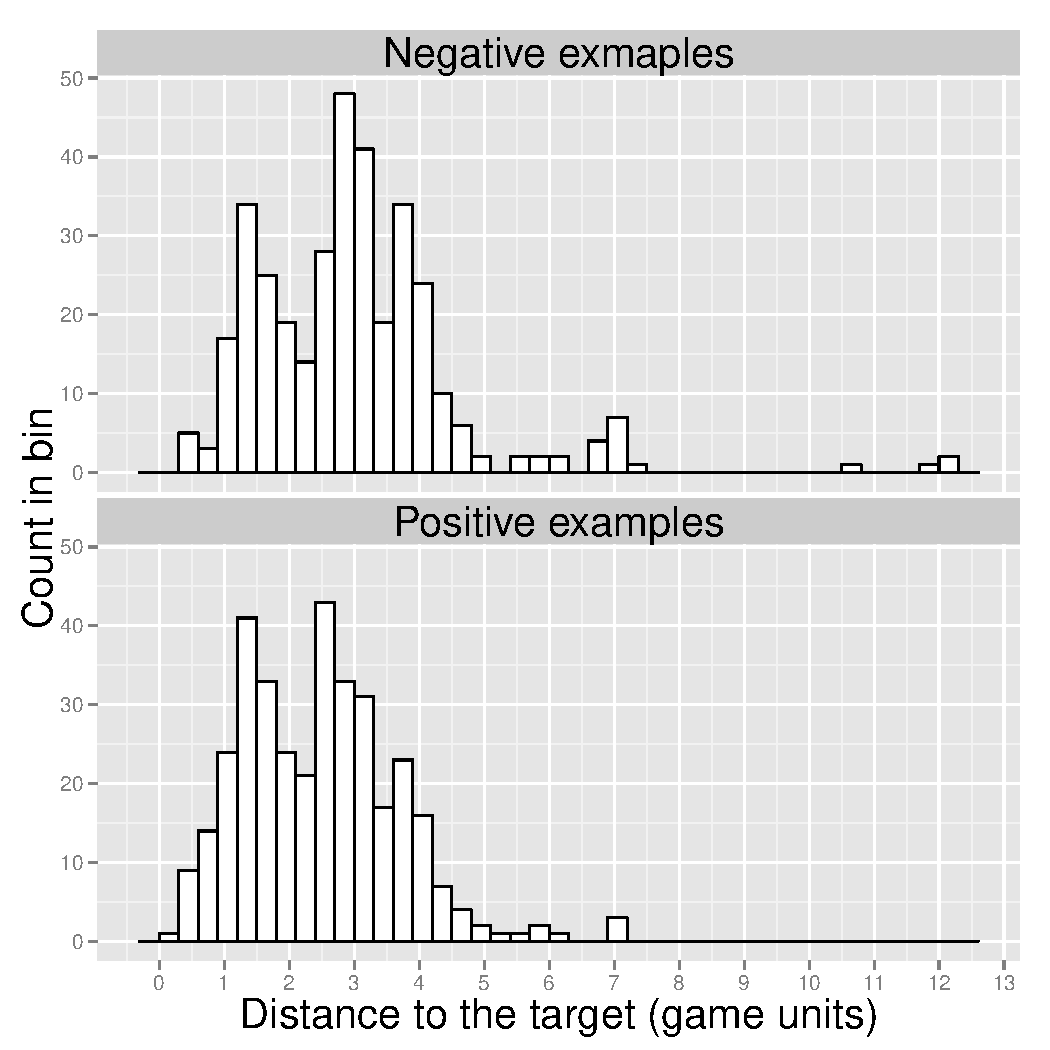
\includegraphics[page=1,width=0.8\textwidth]{Images/fref_distrib}
	\caption{Histogram of attribute distance to the target}
	\label{fig:fref-distrib-dist}
\end{figure}

\begin{figure}[!htbp]
  \centering
	\includegraphics[page=2,width=0.8\textwidth]{Images/fref_distrib}
	\caption{Histogram of attribute angle to the target}
	\label{fig:fref-distrib-angle}
\end{figure}

\begin{figure}[!htbp]
  \centering
	\includegraphics[page=3,width=0.8\textwidth]{Images/fref_distrib}
	\caption{Histogram of attribute whether the target is visible}
	\label{fig:fref-distrib-visib}
\end{figure}

\begin{figure}[!htbp]
  \centering
	\includegraphics[page=4,width=0.8\textwidth]{Images/fref_distrib}
	\caption{Histogram of attribute number of distractors}
	\label{fig:fref-distrib-distractors}
\end{figure}

\begin{figure}[!htbp]
  \centering
	\includegraphics[page=5,width=0.8\textwidth]{Images/fref_distrib}
	\caption{Histogram of attribute number of distracting buttons}
	\label{fig:fref-distrib-distbuttons}
\end{figure}

\begin{figure}[!htbp]
  \centering
	\includegraphics[page=6,width=0.8\textwidth]{Images/fref_distrib}
	\caption{Histogram of attribute number of distracting buttons with lesser angle}
	\label{fig:fref-distrib-distangles}
\end{figure}

\FloatBarrier

\section{Histograms for chains ML}
\begin{figure}[!htbp]
  \centering
	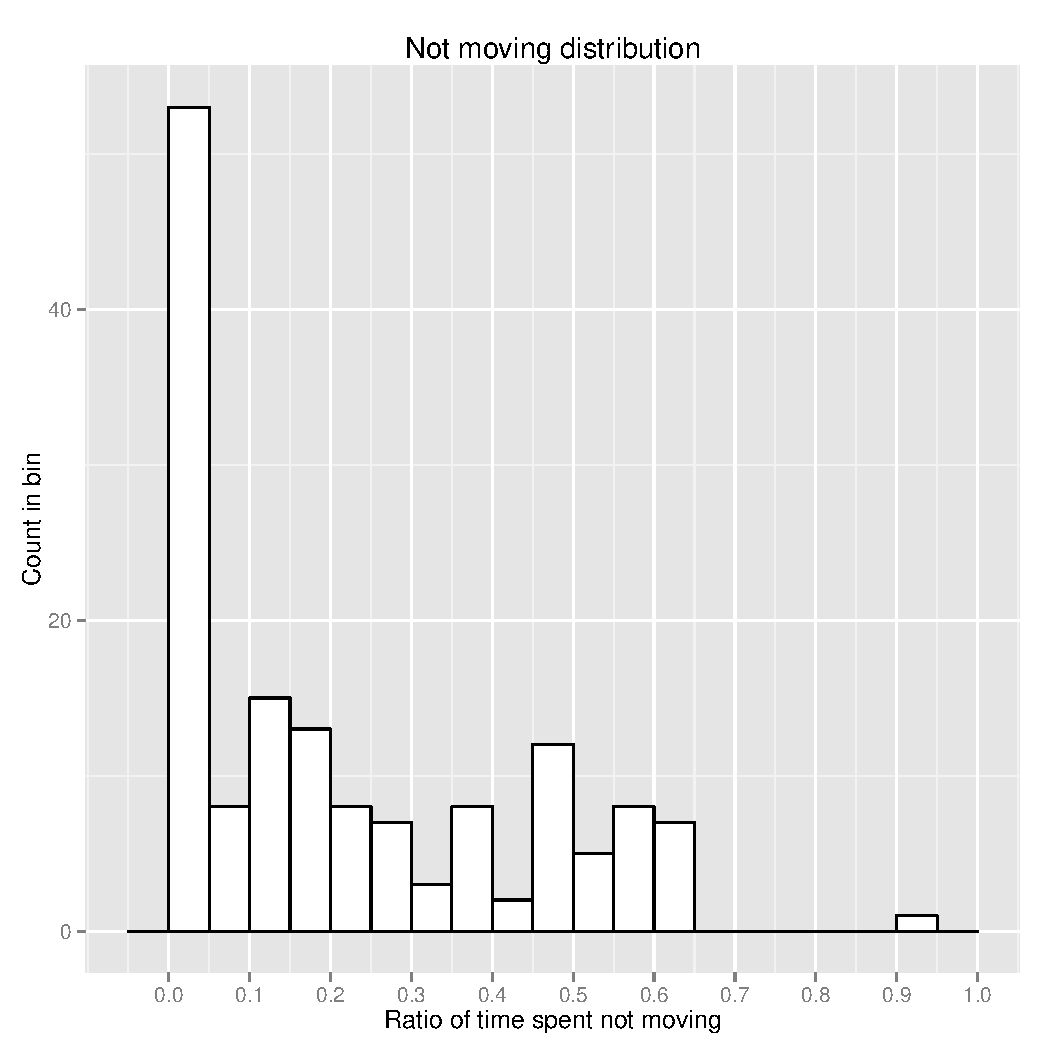
\includegraphics[page=1,width=0.8\textwidth]{Images/chains_features_ML}
	\caption{Histogram of attribute time spent not moving}
	\label{fig:chains-distrib-stop}
\end{figure}

\begin{figure}[!htbp]
  \centering
	\includegraphics[page=2,width=0.8\textwidth]{Images/chains_features_ML}
	\caption{Histogram of attribute time spent rotating}
	\label{fig:chains-distrib-rotate}
\end{figure}

\begin{figure}[!htbp]
  \centering
	\includegraphics[page=3,width=0.8\textwidth]{Images/chains_features_ML}
	\caption{Histogram of attribute objects in the room}
	\label{fig:chains-distrib-objects}
\end{figure}

\begin{figure}[!htbp]
  \centering
	\includegraphics[page=4,width=0.8\textwidth]{Images/chains_features_ML}
	\caption{Histogram of attribute buttons in the room}
	\label{fig:chains-distrib-buttons}
\end{figure}

\begin{figure}[!htbp]
  \centering
	\includegraphics[page=5,width=0.8\textwidth]{Images/chains_features_ML}
	\caption{Histogram of attribute landmarks in the room}
	\label{fig:chains-distrib-landmarks}
\end{figure}

\begin{figure}[!htbp]
  \centering
	\includegraphics[page=6,width=0.8\textwidth]{Images/chains_features_ML}
	\caption{Histogram of attribute very close buttons to the target}
	\label{fig:chains-distrib-veryclose}
\end{figure}

\begin{figure}[!htbp]
  \centering
	\includegraphics[page=7,width=0.8\textwidth]{Images/chains_features_ML}
	\caption{Histogram of attribute buttons on the same wall as the target}
	\label{fig:chains-distrib-samewall}
\end{figure}

\begin{figure}[!htbp]
  \centering
	\includegraphics[page=8,width=0.8\textwidth]{Images/chains_features_ML}
	\caption{Histogram of attribute close buttons to the target}
	\label{fig:chains-distrib-close}
\end{figure}

\begin{figure}[!htbp]
  \centering
	\includegraphics[page=9,width=0.8\textwidth]{Images/chains_features_ML}
	\caption{Histogram of attribute far buttons from the target}
	\label{fig:chains-distrib-far}
\end{figure} % příloha 1: vložená z externího souboru
%\input{priloha2.tex}
%\input{priloha3.tex}


\end{document} % SEM NESAHEJTE!
